\documentclass[11pt,a4paper]{article}
\usepackage[utf8]{inputenc}
\usepackage[T1]{fontenc}
\usepackage{mathpazo}
\usepackage{amsmath,amssymb}
\usepackage[a4paper,margin=2.4cm]{geometry}
\usepackage{graphicx}
\usepackage{pdflscape}
\usepackage{booktabs,array,longtable,tabularx}
\usepackage{xcolor}
\usepackage[numbers,square,sort&compress]{natbib}
\usepackage[most]{tcolorbox}
\usepackage{caption}
\usepackage{enumitem}
\usepackage{fancyhdr}
\usepackage{microtype}
\usepackage[colorlinks=true,linkcolor=bleu!70!black,citecolor=bleu!70!black,urlcolor=bleu!70!black]{hyperref}

\graphicspath{{./}{figures/}}
\definecolor{bleu}{HTML}{2A78D6}
\definecolor{orange}{HTML}{EB6834}
\definecolor{vert}{HTML}{139062}
\definecolor{gris}{HTML}{52514E}

% macros pour la bibliographie (BibTeX de l'auteur)
\newcommand{\apj}{Astrophys. J.}
\newcommand{\apjl}{Astrophys. J. Lett.}
\newcommand{\aj}{Astron. J.}

% unités et symboles
\newcommand{\Rt}{\ensuremath{R_\oplus}}
\newcommand{\Mt}{\ensuremath{M_\oplus}}
\newcommand{\ML}{\ensuremath{M_L}}
\newcommand{\LEM}{\ensuremath{L_{\rm EM}}}
\newcommand{\Req}{\ensuremath{R_{\rm eq}}}
\newcommand{\qB}{\ensuremath{q_B}}
\newcommand{\wt}{\ensuremath{\tilde\omega}}

% statuts
\newcommand{\stCalc}{\textcolor{vert}{\textbf{Computed}}}
\newcommand{\stSup}{\textcolor{orange}{\textbf{Assumed}}}
\newcommand{\stOuv}{\textcolor{gris}{\textbf{Open}}}
\newcommand{\stNon}{\textcolor{red!70!black}{\textbf{Not satisfied}}}

% encadrés
\newtcolorbox{simple}{enhanced,breakable,colback=bleu!5,colframe=bleu!70!black,boxrule=0.5pt,arc=2pt,left=7pt,right=7pt,top=4pt,bottom=4pt,fonttitle=\bfseries\small,title={In plain terms}}
\newtcolorbox{encadre}[1]{enhanced,breakable,colback=orange!6,colframe=orange!85!black,boxrule=0.5pt,arc=2pt,left=7pt,right=7pt,top=4pt,bottom=4pt,fonttitle=\bfseries\small,title={#1}}

\captionsetup{font=small,labelfont=bf,labelsep=period,width=0.94\linewidth}
\renewcommand{\figurename}{Figure}
\renewcommand{\tablename}{Table}
\renewcommand{\contentsname}{Contents}
\renewcommand{\refname}{References}
\renewcommand{\bibsection}{\section*{References}\addcontentsline{toc}{section}{References}}
\renewcommand{\appendixname}{Appendix}
\setlength{\parskip}{4pt}
\setlength{\parindent}{0pt}
\renewcommand{\arraystretch}{1.12}
\setcounter{tocdepth}{2}

\pagestyle{fancy}
\fancyhf{}
\fancyhead[L]{\small M. Debailleul --- A retrodictive theory of the origin of the Moon}
\fancyhead[R]{\small\thepage}
\fancyfoot[C]{\footnotesize \copyright{} 2026 Michel Debailleul --- License CC BY 4.0 --- ORCID 0009-0003-1222-1433}
\renewcommand{\headrulewidth}{0.3pt}

\hypersetup{pdftitle={A retrodictive theory of the origin of the Moon: a secondary circumterrestrial disk redistributed by the retrograde flyby of a rocky planet},pdfauthor={Michel Debailleul},pdfsubject={Origin of the Moon},pdfkeywords={origin of the Moon, secondary disk, Roche limit, retrograde flyby, tides}}

\begin{document}

\thispagestyle{empty}
\begin{center}
{\LARGE\bfseries A retrodictive theory of the origin of the Moon:\\[4pt]
a secondary circumterrestrial disk redistributed\\[4pt]
by the retrograde flyby of a rocky planet\par}
\vspace{16pt}
{\large\bfseries Michel Debailleul\par}
\vspace{3pt}
Geophysicist\\
M.Sc.: Universit\'e libre de Bruxelles (ULB)\\
Independent Researcher\\
ORCID: \href{https://orcid.org/0009-0003-1222-1433}{0009-0003-1222-1433}\\
\href{mailto:michel.debailleul@yahoo.fr}{michel.debailleul@yahoo.fr}\par
\vspace{6pt}
October 2026\par
\smallskip DOI: \href{https://doi.org/10.5281/zenodo.23391968}{10.5281/zenodo.23391968}\par
\end{center}
\vspace{4pt}

\begin{encadre}{Abstract}
\small
The Moon is a datum, and the question is retrodictive: which physical pathways lead to it without a giant impact? The pathway examined starts from a young, hot proto-Earth, \emph{soft but never liquid}, flattened and inflated by a 6~h rotation, surrounded by a disk of material that has not yet formed a satellite. A second rocky planet, planet~$B$, passes close to the Earth against its rotation, without touching it and without giving it any material: it acts by gravity alone. It reworks the disk (about $47\,\%$ stays bound to the Earth, $3.5$ times more than for a flyby in the sense of the rotation), tilts the Earth's axis, and carries away some of the angular momentum of its rotation. The bound material assembles into a body of about one lunar mass in every realization computed; it is kept in four realizations out of ten, when its orbit settles beyond the corotation radius, and tides carry it to the present lunar distance in $4.5$ billion years.

\smallskip
\textbf{The isotopic correspondence.} Since planet~$B$ supplies no material, the Moon is made of terrestrial material: the Earth--Moon isotopic identity (O, Ti, Cr, $^{182}$W) and the depletions in V, Cr, Mn are expected from the outset, where the giant impact has to explain them after the fact.

\smallskip
\textbf{Angular momentum.} The bound system holds $0.21\,\LEM$ more than the present Earth--Moon pair. Braking by planet~$B$, the solar tide and the evection resonance each remove only part of it; computed together on a single trajectory, they close the budget at $\pm0.05\,\LEM$ in about a quarter to a third of the trajectories explored, and at $\pm0.08\,\LEM$ in about two fifths to two thirds, under two conditions that the text states: a weak terrestrial tide early in the history, as befits a soft body, and a slow contraction of the proto-Earth. These percentages describe the parameter grid studied, not a probability.

\smallskip
The results are necessary conditions or families of solutions, not facts; the limits are stated section by section.

\smallskip
\textbf{Keywords.} origin of the Moon; secondary disk; Roche limit; retrograde flyby; soft body; tides; evection; retrodiction.
\end{encadre}

\newpage
\tableofcontents
\newpage

% =====================================================================
\section{The principle: reading the origin of the Moon backwards}
\label{sec:principe}

\begin{simple}
Picture the young Earth, hot, soft and swollen, surrounded by a ring of debris that has not yet become a moon. A second planet, which we call planet~$B$, passes very close, against the rotation of the Earth, without touching it. It brings nothing; it only pulls. When it has gone, a good part of the ring still orbits the Earth, on reworked orbits, and within a few weeks this material assembles into a single body the size of the Moon. Whether this body lasts depends on where its orbit settles: too close to the Earth, the tide makes it fall; far enough out, the tides push it outwards for billions of years, up to the present distance. Since nothing foreign entered the story, the Moon is made of terrestrial material.
\end{simple}

\subsection{The Moon as a datum}

Every theory of the origin of the Moon, the giant impact included, is a reconstruction. The event cannot be replayed: one computes its consequences and compares them with what remains. And what remains is known precisely. The Moon is there, with its mass, its distance, its orbit, its isotopic composition, its poverty in volatiles and in metallic iron, and the angular momentum of the Earth--Moon system as a whole (Table~\ref{tab:contraintes}). These are the data of the problem.

The approach followed here is called \emph{retrodictive}: it goes back from the result to its possible causes. It has three concrete consequences. One starts from the Moon, not from an event supposed to have produced it. One looks for the set of pathways that physics allows, and asks how far the Moon as it is constrains them. Finally, no actor is added to manufacture a result: planet~$B$ passes, it redistributes matter and angular momentum, nothing more.

\begin{table}[htbp]
\centering
\caption{The Moon as it is: the main constraints. These are targets to reach, not results of this document.\label{tab:contraintes}}
\small
\begin{tabular}{>{\raggedright\arraybackslash}p{3.2cm}>{\raggedright\arraybackslash}p{7.6cm}>{\raggedright\arraybackslash}p{4.2cm}}
\toprule
Family & Value & Source \\
\midrule
Mass and architecture & $M_L/\Mt\simeq1.23\times10^{-2}$; a single large satellite & \citep{Williams2014} \\
Orbit & distance $\simeq60\,\Rt$; inclination of $5.1^\circ$ to the ecliptic & --- \\
Rotation of the Earth & obliquity of $23.4^\circ$, $24$~h day & --- \\
Angular momentum & Earth--Moon total $\LEM\simeq3.5\times10^{34}$~kg\,m$^2$\,s$^{-1}$ & \citep{Canup2004,CanupAsphaug2001} \\
Isotopes & O, Ti, Cr, W almost identical to those of the Earth & \citep{Young2016,Zhang2012,Dauphas2017,Kruijer2015,Touboul2015} \\
Volatiles and water & depleted, but lunar water is not zero & \citep{Saal2008,Saal2013,Hauri2011} \\
Iron & core of $1$--$2\,\%$ of the mass; density $3.34$~g\,cm$^{-3}$ & --- \\
Age & formed at least $4.51$ billion years ago & \citep{Barboni2017} \\
\bottomrule
\end{tabular}
\end{table}

\subsection{The story in five stages}

Before going into detail, here is the whole story, with the figures that the document establishes.

\begin{enumerate}[leftmargin=1.6em,itemsep=3pt]
\item \textbf{Before the flyby.} The proto-Earth is hot, soft and swollen: it rotates in $6$~h and its equatorial radius is $1.60\,\Rt$. Around it, a disk of $4.5$ to $5.4$ lunar masses extends from $2.9$ to $5\,\Rt$. It is dispersed, hot, and its pieces do not stick.
\item \textbf{The flyby.} Planet~$B$ ($0.95$ Earth mass) passes at $3.0\,\Rt$ from the center of the Earth, against its rotation, with a speed of $2$~km\,s$^{-1}$ far from the Earth. The passage lasts a few hours, of which about $86$ minutes within $4\,\Rt$. It lightens the surface under planet~$B$, keeps about $47\,\%$ of the disk around the Earth on inclined orbits, tilts the Earth's axis and removes a little of its rotation.
\item \textbf{The assembly.} Within a few weeks, the redistributed material, which now sticks, assembles into a dominant body of about one lunar mass ($1.2$ to $1.7$ after one year).
\item \textbf{The retention.} The body is kept only if its orbit settles beyond the corotation radius of the Earth ($2.6\,\Rt$). In four realizations out of ten this is the case; in four others, the body falls onto the Earth between day $65$ and day $175$.
\item \textbf{The tides.} Over $4.5$ billion years, the tides push the kept satellite out to $60$--$62\,\Rt$ and slow the Earth down. The bound system then holds $0.21\,\LEM$ more than the present Earth--Moon pair; it is this excess that Section~\ref{sec:AM} examines.
\end{enumerate}

\subsection{The method in four steps}

The document follows four steps, summarized in Figure~\ref{fig:chaine}. One first fixes the datum: the Moon as it is. One then lays down explicit, numbered conditions, each of which is stated to be assumed or computed (Section~\ref{sec:decor}). One then computes the physical chain from these conditions to a satellite, keeping controls: a flyby in the sense of the rotation, and a calculation without planet~$B$ (Sections~\ref{sec:methode} and~\ref{sec:survol}). Finally one compares the result with the Moon gate by gate, saying which gates are passed, which show a gap and which remain to be computed (Section~\ref{sec:discussion}).

\begin{figure}[htbp]
\centering
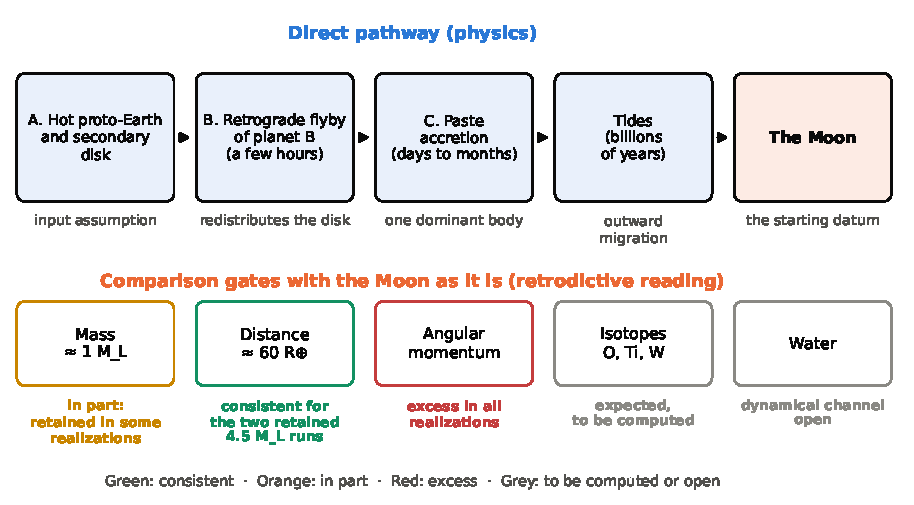
\includegraphics[width=\linewidth]{fig_chaine.pdf}
\caption{The logic of the theory. Top, the direct pathway: proto-Earth and secondary disk (phase~A, assumed starting point), retrograde flyby of planet~$B$ (phase~B), assembly of the satellite in paste (phase~C), tides. Bottom, the gates of comparison with the Moon as it is.\label{fig:chaine}}
\end{figure}

\subsection{What ``possible'' means}

To say that a pathway is possible is to establish that, under explicit conditions, the laws of physics leave it open and that its result falls within the orders of magnitude of the datum. It is not to say that the Moon formed this way. The results of this document are therefore of two kinds. They are \emph{necessary conditions}: for instance, read backwards, the Moon requires the Earth to have rotated with a certain angular momentum; other values of the free parameters can lead to the same final state, and the calculation does not say which one occurred. Or they are \emph{families of solutions}, whose edges are given when they are known. The same criterion holds for any other origin of the Moon.

So that the reader always knows where he stands, each important statement carries one of three statuses: \stCalc{} (result of the calculations of this document, in the model described), \stSup{} (input datum or hypothesis, not demonstrated here), \stOuv{} (defined but not computed).

% =====================================================================
\section{The physical setting}
\label{sec:decor}

This section describes, in words, the actors of the theory and the hypotheses that define them. The calculations that rest on them come afterwards.

\subsection{A hot, soft, flattened proto-Earth}
\label{sec:chaude}

A planet that grows by accretion converts into heat the energy of the material that falls on it. For an Earth mass and radius, this amounts to about $3.7\times10^7$~J per kilogram, nearly a hundred times what is needed to melt a silicate. The accretion energy is therefore sufficient, in order of magnitude, to melt the whole planet and vaporize part of it, \emph{if it is sufficiently retained}. Magma-ocean models show that a vapor envelope can slow the cooling considerably \citep{ElkinsTanton2012,Hamano2013,Lebrun2013,Rubie2015}. The proto-Earth is therefore hot, and the theory assumes it so (hypothesis H1).

\textbf{A soft body, never liquid.} The proto-Earth of this theory is a \emph{soft} body: a pasty material, like a thick modeling clay, not a liquid. This precision matters for what follows. A liquid follows a tide without friction; a cold solid hardly deforms; a soft material deforms under the tide and rubs, so that its behavior is neither that of one nor of the other. The tide raised in a soft body is not that of a solid body, which has two consequences to which we return: the tide is weak at the beginning of the history, and the dissipation depends on the viscosity of the material. The passage of planet~$B$ changes nothing of this soft character; it lasts a few hours and the Earth does not cool during that time.

\textbf{Flattened and swollen.} A soft body that rotates flattens at the poles and swells at the equator. With a rotation of $6$~h, we adopt an equatorial radius $\Req=1.60\,\Rt$ (and $1.52\,\Rt$ for a rotation of $5$~h). These radii are \emph{input hypotheses}, not computed structures; Section~\ref{sec:poids} shows why the theory requires them. The rotation of $5$ to $6$~h is also assumed (H2): accretion can supply it, without an impact. An objection exists: \citet{DonesTremaine1993} showed that the steady accretion of small bodies does not give a planet like the Earth its present rotation rate. H2 therefore remains a hypothesis. The retrodiction of Section~\ref{sec:AM} starts from the Moon and does not use it, but the excess of angular momentum that it quantifies depends on it.

\begin{table}[htbp]
\centering
\caption{Figure of the proto-Earth for the two reference cases (computed from H1 and H2). The rotation number compares the rotation speed with that at which an equatorial particle would orbit; it would be~1 at break-up.\label{tab:forme}}
\small
\begin{tabular}{lcc}
\toprule
Quantity & 5 h, $1.52\,\Rt$ & 6 h, $1.60\,\Rt$ \\
\midrule
Rotation number & $0.53$ & $0.47$ \\
Flattening (polar / equatorial radius) & $0.88$ & $0.90$ \\
Remaining equatorial gravity & $72\,\%$ & $78\,\%$ \\
Mean density & $1.8$--$1.9$~g\,cm$^{-3}$ & $1.5$~g\,cm$^{-3}$ \\
Corotation radius & $2.33\,\Rt$ & $2.63\,\Rt$ \\
\bottomrule
\end{tabular}
\end{table}

The \emph{corotation radius} of Table~\ref{tab:forme} is the distance at which a body in orbit turns exactly as fast as the Earth. It plays a central role further on: a satellite that settles beyond this radius is pushed away by the tide, a satellite that settles inside it is pulled towards the Earth.

\subsection{The secondary disk and the Roche limit}
\label{sec:roche}

Around the proto-Earth lies a \emph{secondary disk}: a reservoir of material born at the same time as it, which has not yet formed a satellite. The theory places it beyond the \emph{Roche limit}. This is the distance inside which the tide of the planet tears a fluid body apart faster than its own gravity can gather it; beyond it, bodies can grow \citep{SalmonCanup2012}. For material of lunar density ($3.34$~g\,cm$^{-3}$), this limit is at $2.90\,\Rt$. It depends only on the mass of the Earth and the density of the satellite, \emph{not} on the swelling of the proto-Earth. Lighter material has a more distant limit: $3.15\,\Rt$ at $2.6$~g\,cm$^{-3}$, $3.79\,\Rt$ at $1.5$~g\,cm$^{-3}$.

The disk extends from the Roche limit to about $5\,\Rt$. Its surface density increases outwards, as expected when the transport of angular momentum spreads material to large radii. It is thick in latitude, in the intertropical band ($\pm26^\circ$), because the passage of planet~$B$ is inclined by $25^\circ$ and it is there that its tide is felt. Its formation (phase~A) is not computed: its total mass, from $4$ to $5.4$ lunar masses, is a parameter (H3). Figure~\ref{fig:zones} gives the map of distances.

\begin{figure}[htbp]
\centering
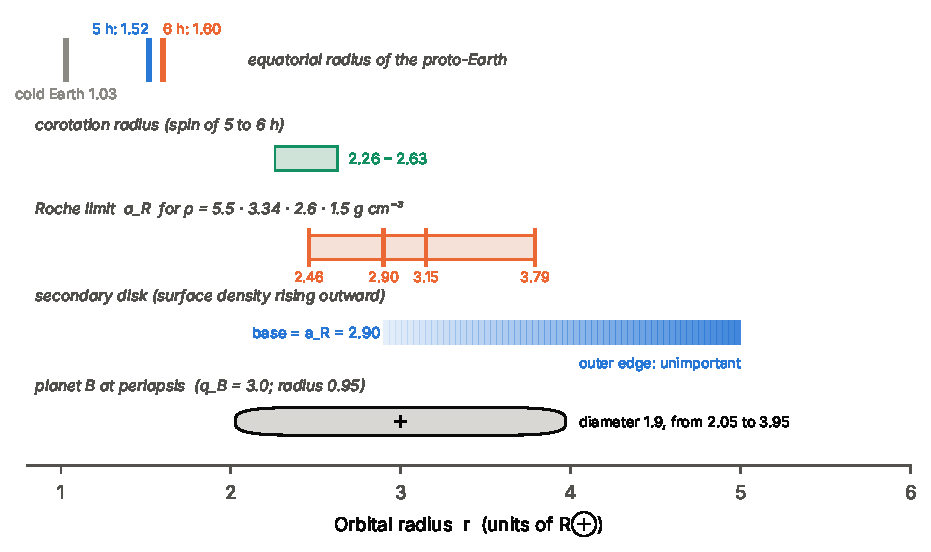
\includegraphics[width=\linewidth]{fig_zones.pdf}
\caption{Radial map of the system, in Earth radii: equatorial radii of the proto-Earth (5~h, 6~h), corotation radius, extent of the Roche limit according to the density of the material, secondary disk (surface density increasing outwards) and planet~$B$ at its closest point.\label{fig:zones}}
\end{figure}

\textbf{A disk first non-sticky, then pasty (proposition P2).} Until the passage of planet~$B$, the disk is bathed in the gas of the young Sun, in the vapor of the magma ocean and in the radiation of the proto-Earth, whose surface is at $2000$--$3000$~K. Under these conditions bodies that touch bounce or erode instead of merging: the disk stays dispersed. The passage takes place during the gas phase, in the first million years of the Solar System \citep{Weiss2021,Mamajek2009}. After the passage, the redistributed material is treated as a \emph{soft paste}: two pieces that touch stick together (H4). A corollary on age: the Moon forms shortly after the Earth, and the ages of $4.51$ and $4.46$ billion years \citep{Barboni2017,Greer2023} date the core--mantle differentiation and the crystallization of the lunar magma ocean, not the accretion.

\textbf{A disk poor in metallic iron (proposition P1).} The Moon has little metallic iron, and its density is $3.34$~g\,cm$^{-3}$. The theory assumes that the disk was depleted in metal before the passage: the metal, being denser, joined the core of the proto-Earth. This proposition is not computed; it has a testable consequence on the elements that follow iron (Ni, Co, W).

\subsection{Planet~$B$ and what it does}
\label{sec:B}

Planet~$B$ is a rocky planet of $0.95$ Earth mass, covered with a thin film of ice (H5). It is a little denser than the Earth ($6.1$~g\,cm$^{-3}$) rather than larger, which lets it pass close to the Earth without breaking up: at $3.0\,\Rt$ from the center, it keeps a margin of $18\,\%$ over the contact distance with a proto-Earth of $1.60\,\Rt$. It follows an open trajectory (a hyperbola), at $2$~km\,s$^{-1}$ far from the Earth and $9.2$~km\,s$^{-1}$ at its closest point. It is \emph{retrograde}, that is, against the rotation of the Earth, and inclined by $25^\circ$ to the equator (H6).

\textbf{No material is transferred (H7).} Planet~$B$ supplies no material to the proto-Earth or to the satellite being formed. It acts by gravity alone. The only thing it leaves is the water vapor of its ice film, which arrives mostly on the Earth (H8, Section~\ref{sec:eau}). This rule is the heart of the isotopic character of the theory (Section~\ref{sec:isotopes}).

\textbf{Three effects, all gravitational.} During the few hours of the flyby, planet~$B$ acts in three ways.
\begin{enumerate}[leftmargin=1.6em,itemsep=2pt]
\item It \emph{redistributes the material of the disk}: part falls onto the Earth, part stays bound on new, more inclined orbits, part escapes.
\item It \emph{tilts the rotation axis} of the Earth, through its attraction on the equatorial bulge.
\item It \emph{carries away a little of the angular momentum} of the rotation of the Earth: the tide it raises brakes the rotation, and the angular momentum thus removed from the Earth passes into the motion of planet~$B$.
\end{enumerate}
The following phases (assembly of the satellite, tides) keep or transfer what remains; they remove almost nothing. We shall see that the amount removed by the third effect depends on the nature of the material of the proto-Earth, and that it is modest.

\textbf{Why retrograde.} At its closest point, planet~$B$ moves at an angular speed of $4.8\times10^{-4}$~s$^{-1}$, while the material of the disk rotates at $2.4\times10^{-4}$~s$^{-1}$ at $3\,\Rt$ and at $1.1\times10^{-4}$~s$^{-1}$ at $5\,\Rt$. In the sense of the rotation (prograde), planet~$B$ slowly catches up with the material, and the same parcels are pulled coherently for a long time: they are torn away. Against the rotation (retrograde), planet~$B$ meets the material head on: each parcel receives a brief kick, and the kicks accumulate less. The retrograde passage therefore \emph{rearranges} the orbits without carrying the disk away. The numerical contrast is given in Section~\ref{sec:phaseB}.

\textbf{Geometry.} The argument of periapse $\omega_B=90^\circ$ places the closest point to the Earth at the top of the orbit, at latitude $+25^\circ$ above the equator (Figure~\ref{fig:geometry}). Planet~$B$ therefore passes \emph{above} the disk, about $3\,\Rt$ from the Earth, and its center crosses the plane of the disk only after leaving it, about $6\,\Rt$ from the Earth (the disk stops at $5\,\Rt$). An orbit with $\omega_B=0$ would instead pass in the plane of the disk; this is not the hypothesis of the theory.

\begin{table}[htbp]
\centering
\caption{Planet~$B$ and the geometry of the reference passage (computed, unperturbed hyperbolic orbit).\label{tab:B}}
\small
\begin{tabular}{lc}
\toprule
Quantity & Value \\
\midrule
Mass, radius, density & $0.95\,\Mt$, $0.95\,\Rt$, $6.1$~g\,cm$^{-3}$ \\
Surface gravity & $1.05\,g_\oplus$ \\
Closest-point distance $\qB$ & $3.0\,\Rt$ \\
Speed at infinity, speed at the closest point & $2$ and $9.24$~km\,s$^{-1}$ \\
Eccentricity of the hyperbola & $1.098$ \\
Inclination to the equator (retrograde), argument of periapse & $25^\circ$, $90^\circ$ \\
Height of the center of planet~$B$ above the equator at periapse & $1.27\,\Rt$ \\
Distance at which its center crosses the equatorial plane & $6.3\,\Rt$ \\
\bottomrule
\end{tabular}
\end{table}

\begin{figure}[htbp]
\centering
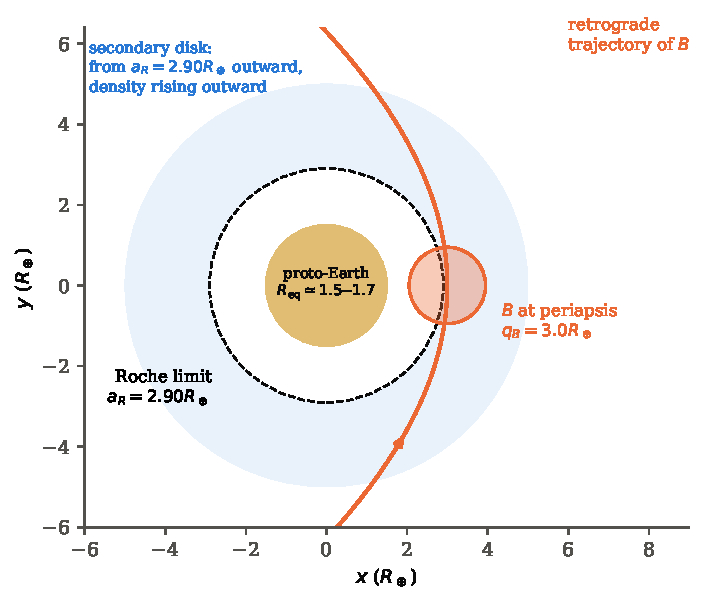
\includegraphics[width=0.78\linewidth]{fig_geometry.pdf}
\caption{Geometry of the passage in the equatorial plane of the Earth (to scale; the real trajectory is inclined by $25^\circ$). The secondary disk starts at the Roche limit ($2.90\,\Rt$, dashed). Planet~$B$ reaches its closest point at $3.0\,\Rt$, at the base of the disk, moving against the rotation of the Earth.\label{fig:geometry}}
\end{figure}

\subsection{The hypotheses in one table}

Table~\ref{tab:hypotheses} lists the conditions laid down. None is hidden in the code: each is an input datum or a computing rule, and its status is stated.

\begin{table}[htbp]
\centering
\caption{The input hypotheses (H) and propositions (P).\label{tab:hypotheses}}
\small
\begin{tabular}{>{\raggedright\arraybackslash}p{0.9cm}>{\raggedright\arraybackslash}p{10.6cm}>{\raggedright\arraybackslash}p{2.9cm}}
\toprule
No. & Statement & Status \\
\midrule
H1 & Proto-Earth heated by its accretion, soft and not liquid, flattened and swollen to $\Req=1.52\,\Rt$ (5~h) or $1.60\,\Rt$ (6~h) & \stSup \\
H2 & Initial rotation of $5$--$6$~h, supplied by accretion and not by an impact & \stSup \\
H3 & Pre-existing secondary disk, with its base at the Roche limit, in the band $\pm26^\circ$. Its mass is a parameter: from $4.5$ to $5.4$ lunar masses have given a kept satellite & \stSup, mass partly \stCalc \\
H4 & After the flyby, the material is a soft paste: two pieces that touch stick together & \stSup \\
H5 & Planet~$B$: $0.95\,\Mt$, $0.95\,\Rt$, $6.1$~g\,cm$^{-3}$, thin ice film & \stSup \\
H6 & Retrograde flyby, without contact: distance $3.0\,\Rt$, speed $2$~km\,s$^{-1}$ at infinity, inclination $25^\circ$, $\omega_B=90^\circ$ & \stSup \\
H7 & No transfer of material from planet~$B$; it acts by gravity alone & \stSup \\
H8 & The water of the ice film arrives mostly on the Earth & \stSup, channel \stOuv \\
P1 & The disk is depleted in metallic iron before the flyby & \stSup, mechanism \stOuv \\
P2 & Until the flyby, the disk is non-sticky (gas, vapor, radiation); the flyby takes place during the gas phase & \stSup, mechanism \stOuv \\
\bottomrule
\end{tabular}
\end{table}

% =====================================================================
\section{The method in brief}
\label{sec:methode}

The calculation follows three phases, which Figure~\ref{fig:chaine} places on one line. \emph{Phase~A} is the existence of the proto-Earth and its disk; it is assumed, not computed. \emph{Phase~B} is the flyby, which lasts a few hours. \emph{Phase~C} is what follows, from a few days to billions of years.

\textbf{Phase~B: test particles.} The disk is represented by $700$ tracers of equal mass, spread in the intertropical band between the Roche limit and $5\,\Rt$. They are followed while planet~$B$ travels along its hyperbola, from eight periapse distances before the passage to eight after. The tracers do not collide during the few hours of the flyby, which the non-sticky state of the disk before the passage justifies (P2). After the flyby, each tracer is classified according to its energy: bound to the Earth, escaped, or fallen onto the surface. Planet~$B$ is treated as a mass that attracts, nothing more.

\textbf{Phase~C: an $N$-body calculation.} The bound tracers become $700$ small bodies, followed by an $N$-body dynamics code. Bodies that touch merge like a soft paste (H4). The tide of the Earth is included. The result is followed for one year, then, for the realizations that keep a satellite, for five years.

\textbf{Secular tides.} From the state obtained at five years, a model that averages over the fast motions makes the orbit of the satellite and the rotation of the Earth evolve under the tides of the Moon and of the Sun, over $4.5$ billion years. The tidal parameters are calibrated on the dissipation of the present Earth; the distance reached varies slowly with them (a factor $2$ on the dissipation changes the distance by $11\,\%$).

\textbf{Why these tools.} Each tool is chosen for what the phase demands. During the few hours of the flyby, the tracers do not influence one another: they have no time to meet, and the only force that counts is the attraction of the Earth and of planet~$B$. A test-particle calculation is then exact and fast, which allows many geometries to be scanned. After the flyby, on the contrary, the bodies meet, merge and attract one another: an $N$-body calculation is indispensable, and it is slower. Finally, over billions of years it would be impossible to follow each revolution; a model that averages over the fast motions suffices for the slow evolution of the orbits.

\textbf{What is a realization?} The initial distribution of the $700$ tracers is drawn at random, and each draw carries a number, the \emph{seed}. Two seeds give statistically identical disks but different assemblies, because phase~C is chaotic: a small initial difference can change the body that ends up dominating. Each complete calculation is a \emph{realization}. This is why the results of phase~C are given with their scatter and on several realizations, never on a single one.

\textbf{How the calculations are checked.} The fractions of phase~B vary by less than $0.015$ when the resolution, the time step (from $20$ to $5$~s) or the stopping distance (from $30$ to $100\,\Rt$) are changed. The angular momentum of phase~C is conserved to $10^{-4}\,\LEM$ over four years, that of the coupled budget to $10^{-6}\,\LEM$. The calculation of the dissipation of the soft material reproduces to four digits the braking of the constant-lag model when given the same kernel, and recovers the exact solution of a uniform body. The solar tide alone gives back, in the coupled budget, the values of Section~\ref{sec:puits}.

\textbf{Specialized calculations.} Four separate calculations complete the chain: the weight of the magma under planet~$B$; the braking of the rotation and the tilt of the axis, with a model of a soft body (Maxwell rheology); the holding of a rubble pile near the Roche limit; and, new in this version, a \emph{coupled budget} of the angular momentum on a single trajectory (Section~\ref{sec:couple}).

\begin{table}[htbp]
\centering
\caption{Reference configuration. These values are fixed in all calculations, unless a scan is mentioned.\label{tab:config}}
\small
\begin{tabular}{>{\raggedright\arraybackslash}p{4.4cm}>{\raggedright\arraybackslash}p{5.6cm}>{\raggedright\arraybackslash}p{4.6cm}}
\toprule
Quantity & Value & Comment \\
\midrule
Rotation and equatorial radius & $6$~h, $1.60\,\Rt$ (or $5$~h, $1.52\,\Rt$) & hypotheses \\
Planet~$B$ & $0.95\,\Mt$, $0.95\,\Rt$, $6.1$~g\,cm$^{-3}$ & ice film neglected in mass \\
Flyby & distance $3.0\,\Rt$, $2$~km\,s$^{-1}$, $25^\circ$ retrograde, $\omega_B=90^\circ$ & closest point at $+25^\circ$ \\
Disk & from $2.90\,\Rt$ to $5\,\Rt$, increasing surface density, $|\lambda|\le26^\circ$ & mass from $4.0$ to $5.4$ lunar masses \\
Disk material & soft paste at $3\,340$~kg\,m$^{-3}$ & lunar density \\
Tide of the Earth & $k_2=0.032$, lag $959$~s (i.e.\ $k_2/Q\simeq10^{-2}$) & independent calibration \\
\bottomrule
\end{tabular}
\end{table}

% =====================================================================
\section{The flyby and the birth of the satellite}
\label{sec:survol}

This section follows the chain in the order of time: the effect of the flyby on the surface of the Earth, the redistribution of the disk, the assembly of the body, its retention, then its migration to the lunar distance. Each result is followed by what to take from it.

\subsection{The tide of planet~$B$ lightens the magma beneath it}
\label{sec:poids}

At the point of the surface directly beneath planet~$B$, three accelerations combine: the gravity of the Earth, which holds the material; the centrifugal push of the rotation, which lightens it at the equator; and the attraction of planet~$B$, which pulls it upwards. When the pull wins, the material is no longer held to the ground. At a given distance from planet~$B$, one can define a \emph{zero-weight radius}: any point of the surface farther from the center than this radius is unloaded.

At $3.0\,\Rt$, the zero-weight radius is $1.51\,\Rt$ for a rotation of $5$~h and $1.54\,\Rt$ for $6$~h (Figure~\ref{fig:weight}). The surface is therefore unloaded at the closest point only if the equatorial radius of the proto-Earth exceeds these values. Both reference cases satisfy this: at $6$~h and $1.60\,\Rt$, the surface is unloaded over the whole intertropical band, with a margin of $0.01$ to $0.06\,\Rt$. The attraction of planet~$B$ is then $0.97$ times the surface gravity.

\begin{figure}[htbp]
\centering
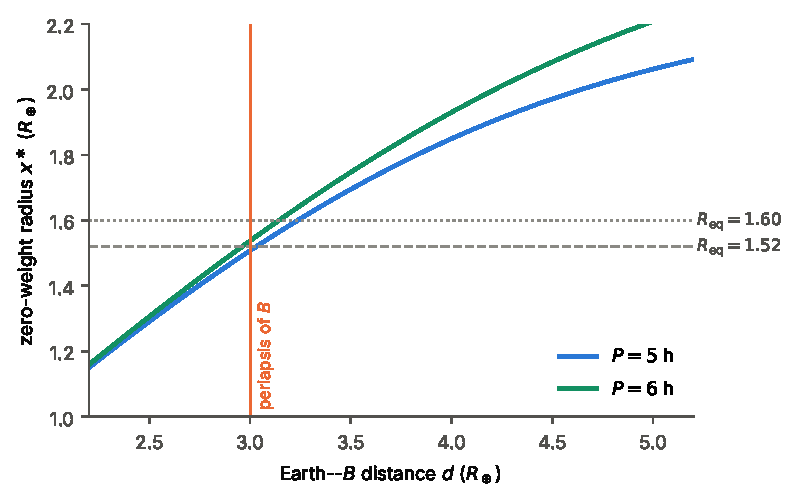
\includegraphics[width=0.85\linewidth]{fig_weight.pdf}
\caption{Zero-weight radius beneath planet~$B$ as a function of its distance, for rotations of $5$~h and $6$~h. A point of the surface is unloaded when the curve passes below the equatorial radius of the proto-Earth. At $3.0\,\Rt$, the curves are at $1.51\,\Rt$ ($5$~h) and $1.54\,\Rt$ ($6$~h).\label{fig:weight}}
\end{figure}

\textbf{To retain.} This condition is precise and refutable: a cold, compact proto-Earth ($\Req\simeq1.03\,\Rt$) would not be unloaded at this distance, and the theory therefore requires an Earth swollen by its heat. The calculation is quasi-static; it fixes the required radius, but does not say how much magma is lifted nor what becomes of it. The calculations that follow do not depend on it.

\subsection{Phase~B: a retrograde passage redistributes the disk}
\label{sec:phaseB}

After the one-hour passage, out of $100$ parts of the disk, about $47$ are still on orbits around the Earth, on orbits inclined by about $31^\circ$; about $21$ have been sent towards the surface of the magma ocean; about $33$ have left the Earth. A passage of the same geometry but in the sense of the rotation would keep only $14$ (Table~\ref{tab:phaseB}, Figure~\ref{fig:phaseB}). The retrograde passage therefore keeps about $3.5$ times more material around the Earth.

\begin{table}[htbp]
\centering
\caption{Fate of the tracers of the disk after the passage (distance $3.0\,\Rt$, $0.95\,\Mt$, disk from $2.90$ to $5\,\Rt$, averages over three seeds of $700$ tracers, scatter of $0.01$--$0.02$). ``Fallen'': fallen onto the Earth; ``bound'': bound to the Earth; ``lost'': having left the Earth; ``periapse $>a_R$'': fraction of the whole disk that is bound and stays outside the zone where a fluid body would be torn apart.\label{tab:phaseB}}
\small
\begin{tabular}{lccccc}
\toprule
Passage & fallen & bound & lost & periapse $>a_R$ & incl. \\
\midrule
Retrograde $25^\circ$ & 0.21 & \textbf{0.47} & 0.33 & 0.15 & $31.5^\circ$ \\
Retrograde coplanar & 0.15 & 0.44 & 0.42 & 0.14 & $20.0^\circ$ \\
Prograde $25^\circ$ & 0.18 & 0.14 & 0.68 & 0.10 & $20.5^\circ$ \\
\bottomrule
\end{tabular}
\end{table}

\begin{figure}[htbp]
\centering
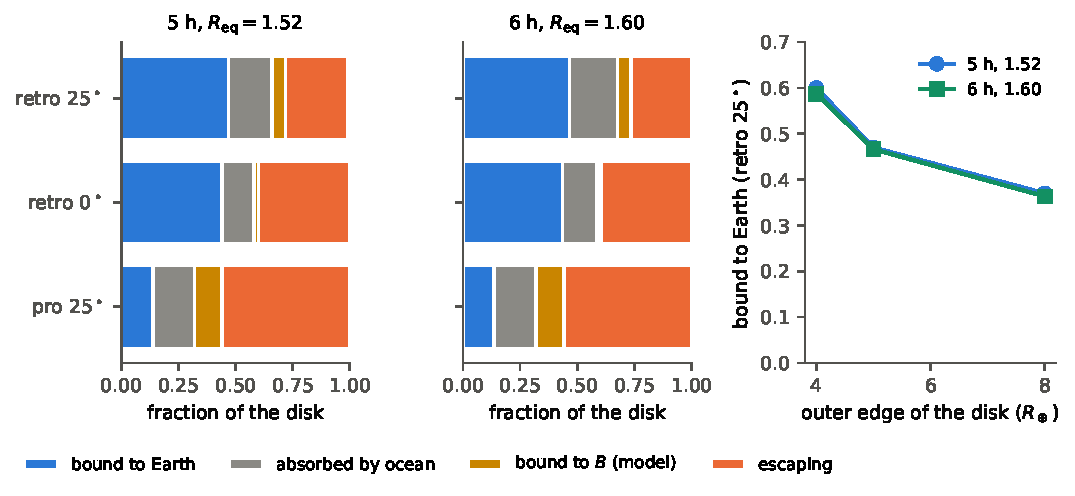
\includegraphics[width=\linewidth]{fig_phaseB.pdf}
\caption{Phase~B. Left and middle: fate of the tracers for the two reference cases and three passages (retrograde at $25^\circ$, retrograde coplanar, prograde at $25^\circ$). Right: fraction of the disk bound to the Earth for the retrograde passage as a function of the outer edge of the disk.\label{fig:phaseB}}
\end{figure}

The result is insensitive to the slope of the surface density (the bound fraction is $0.46$ to $0.48$ for the three slopes tried). It depends, on the other hand, on the outer edge of the disk: $0.60$, $0.47$ and $0.37$ for $4$, $5$ and $8\,\Rt$, because material located beyond the closest point of planet~$B$ is more easily carried away.

A second sorting sheds light on the dynamics. One places $504$ particles on circular orbits between the surface of the swollen Earth and the Roche limit, and looks at where they go (Table~\ref{tab:504}). The retrograde passage at $25^\circ$ is the most efficient: it places $18.5\,\%$ of the reservoir in the ``lunar window'' (bound material, outside the Earth, with a circular radius beyond the Roche limit), keeps $80\,\%$ around the Earth and lets nothing escape. The prograde passage disperses the reservoir: only $4\,\%$ in the window, more than half lost. The efficiency is maximal at $25^\circ$ and does not form a plateau, which anchors the choice of this inclination.

\begin{table}[htbp]
\centering
\caption{Partition of $504$ particles placed between the surface and the Roche limit, after the flyby (average of five grids).\label{tab:504}}
\small
\begin{tabular}{lcccc}
\toprule
Passage & lunar window & bound inner disk & fallen onto the Earth & lost \\
\midrule
Retrograde $20^\circ$ & 0.130 & 0.516 & 0.279 & 0.075 \\
Retrograde $25^\circ$ & \textbf{0.185} & 0.612 & 0.204 & 0.000 \\
Retrograde $30^\circ$ & 0.133 & 0.605 & 0.262 & 0.000 \\
Prograde $25^\circ$ & 0.042 & 0.014 & 0.397 & 0.547 \\
\bottomrule
\end{tabular}
\end{table}

The flyby also \emph{stirs} the disk. The stirring is measured by an index that combines the eccentricity and the inclination of the orbits: it goes from $0.23$ before the flyby to $0.72$ after, and the bound orbits then have a median eccentricity of $0.40$. Neighboring pieces therefore cross at speeds of the order of $0.7$ times the Keplerian speed. This is why the paste rule (H4), which makes bodies stick on contact, is essential to the assembly that follows.

\textbf{To retain.} The retrograde flyby keeps about half of the disk around the Earth, on inclined orbits, against one seventh for the prograde passage. Half a disk bound to the Earth is the raw material of the Moon; a third of this half (about $0.15$ of the disk) is on orbits whose lowest point stays beyond the Roche limit, and can therefore be assembled right away.

\subsection{Phase~C: the paste assembles into a dominant body}
\label{sec:phaseC}

In the first weeks, the redistributed material, which sticks on contact, gathers into a single body. The body then settles near the Roche limit on an almost circular orbit, and its orbital plane slowly approaches the equator (Table~\ref{tab:phaseC}, Figures~\ref{fig:sequence} and~\ref{fig:phaseC}).

\begin{figure}[htbp]
\centering
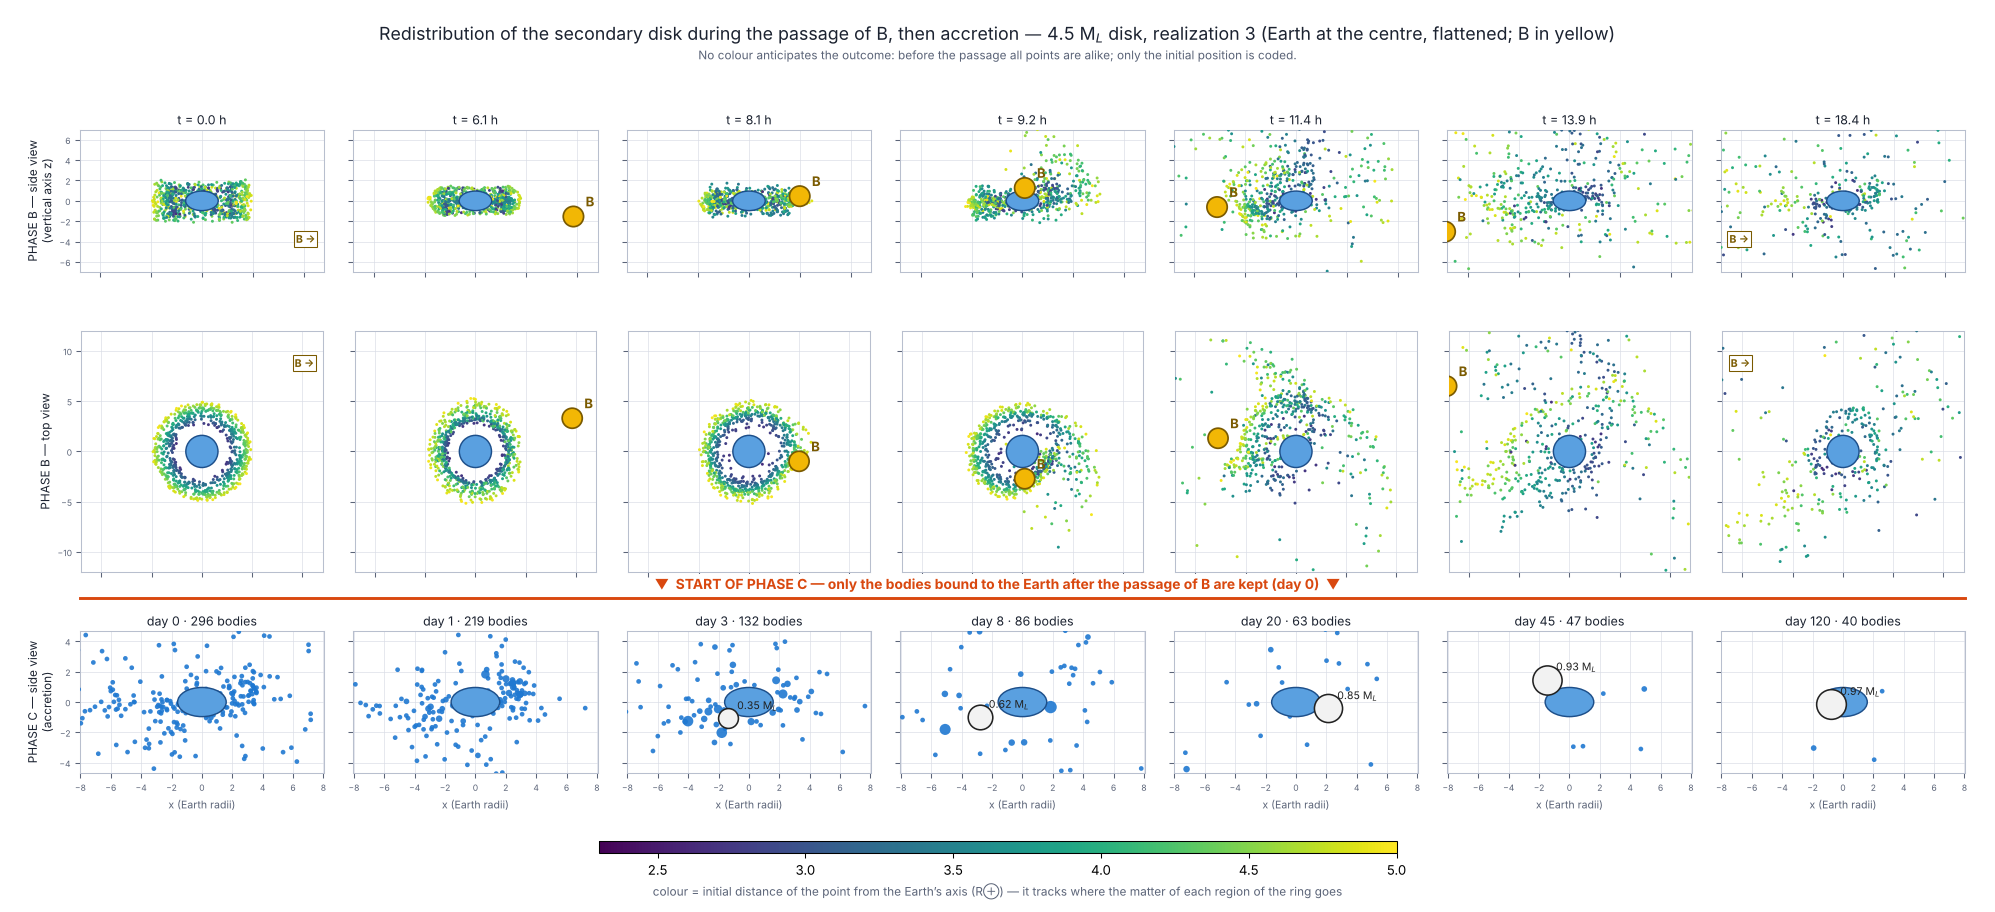
\includegraphics[width=\linewidth]{fig_sequence.png}
\caption{Sequence of phase~C for the reference realization: the material bound after the flyby assembles into a dominant body in a few weeks.\label{fig:sequence}}
\end{figure}

\begin{table}[htbp]
\centering
\caption{Dominant body during the first year (reference realization, seed~0). $M_1$: mass of the dominant body; $a_1$, $e_1$, $i_1$: its semi-major axis, eccentricity and inclination to the equator.\label{tab:phaseC}}
\small
\begin{tabular}{lcccccc}
\toprule
Case & day & $M_1$ ($\ML$) & $a_1$ ($\Rt$) & $e_1$ & $i_1$ ($^\circ$) \\
\midrule
5 h, $1.52\,\Rt$ & 10 & 0.93 & 2.97 & 0.10 & 27.7 \\
 & 90 & 1.20 & 2.77 & 0.10 & 28.1 \\
 & 365 & 1.30 & 3.10 & 0.11 & 12.8 \\
\addlinespace
6 h, $1.60\,\Rt$ & 10 & 1.30 & 3.01 & 0.02 & 26.6 \\
 & 90 & 1.40 & 2.99 & 0.05 & 22.0 \\
 & 365 & 1.43 & 3.17 & 0.08 & 10.4 \\
\bottomrule
\end{tabular}
\end{table}

\begin{figure}[htbp]
\centering
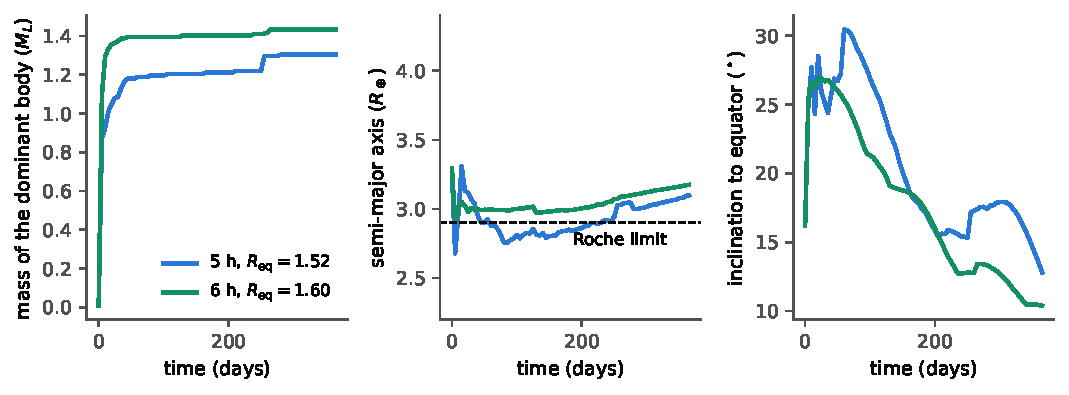
\includegraphics[width=\linewidth]{fig_phaseC.pdf}
\caption{Phase~C with tides (one year) for the two reference cases. Left: mass of the dominant body. Middle: its semi-major axis, compared with the Roche limit. Right: its inclination to the equator.\label{fig:phaseC}}
\end{figure}

\textbf{Dispersion, disk mass, surface rule.} Three additional realizations per case give, after one year, a body of $1.36$ to $1.69$ lunar masses at $5$~h and of $1.23$ to $1.38$ at $6$~h: a body of lunar mass forms in all eight realizations, on an almost circular orbit whose inclination falls to $3$--$13^\circ$. Varying the mass of the disk at $5$~h gives $0.03$, $1.52$ and $1.28$ lunar masses for $2.7$, $5.4$ and $8.1$ lunar masses of disk: with a disk that is too light, the retained material is too sparse to assemble, and the lunar-mass result holds from $5$ to $8$ lunar masses at $5$~h. Finally, in the reference calculation, bodies that touch the surface of the Earth are re-accreted by it (H7 allows it); with the opposite rule, which removes them, the $5$~h case gives $1.60$ lunar masses, that is, the same result.

\textbf{To retain.} A body of $1.30$ to $1.43$ lunar masses dominates from the first weeks, with companions of $0.14$ and $0.02$ lunar mass. The orbit is stable over the year, at about $3$ Earth radii, and the inclination decreases under the effect of the tide from $27^\circ$ to $10^\circ$. The body is not yet on the equator; the tides must bring it there.

\subsection{What the passage changes: the control without planet~$B$}
\label{sec:control}

To know what the flyby changes, phase~C is redone on the same disk without planet~$B$ (Table~\ref{tab:control}, Figure~\ref{fig:temoin}). Left to itself, the disk of $5.4$ lunar masses is dynamically cold and sticky: it collapses within a few days into a single body of $3.5$ to $3.9$ lunar masses, on an almost circular, equatorial orbit, at $4.6$--$4.7\,\Rt$. With planet~$B$, the same starting mass gives a body of $1.3$ to $1.4$ lunar masses, and the system holds $1.35\,\LEM$ instead of about $2.0\,\LEM$.

\begin{table}[htbp]
\centering
\caption{Phase~C after one year, with and without the passage (same disk of $5.4$ lunar masses, same rules). $L$: angular momentum of the dominant body plus rotation of the Earth.\label{tab:control}}
\small
\begin{tabular}{lcccccc}
\toprule
Case & $M_1$ ($\ML$) & $a_1$ ($\Rt$) & $e_1$ & $i_1$ ($^\circ$) & $L$ ($\LEM$) \\
\midrule
5 h, with planet~$B$ & 1.30 & 3.10 & 0.11 & 12.8 & 1.35 \\
5 h, without planet~$B$ & 3.47 & 4.58 & 0.10 & 0.7 & 2.04 \\
6 h, with planet~$B$ & 1.43 & 3.17 & 0.08 & 10.4 & 1.35 \\
6 h, without planet~$B$ & 3.86 & 4.68 & 0.13 & 0.4 & 1.97 \\
\bottomrule
\end{tabular}
\end{table}

\begin{figure}[htbp]
\centering
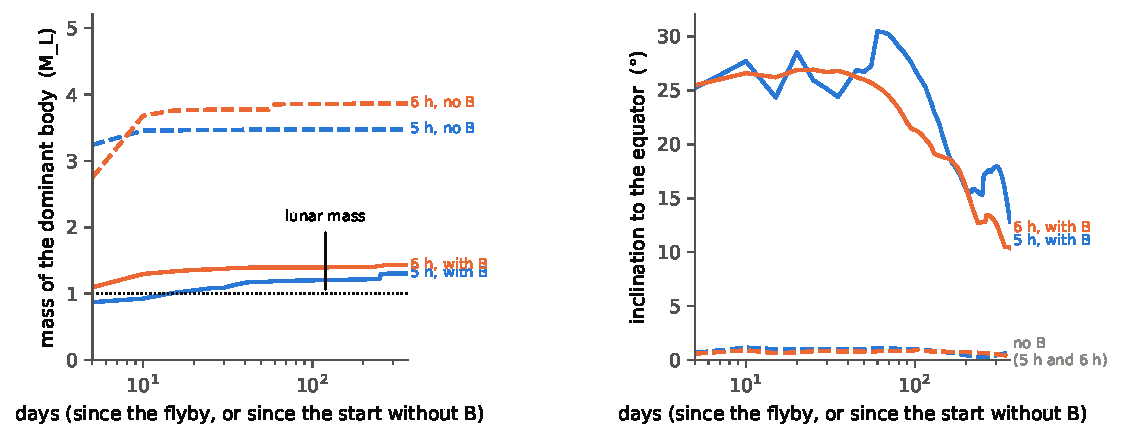
\includegraphics[width=\linewidth]{fig_temoin.pdf}
\caption{Phase~C with and without the passage (same disk, same rules). Left: mass of the dominant body, the dotted line marking the lunar mass. Right: its inclination to the equator. Solid lines: with planet~$B$; dashed: without.\label{fig:temoin}}
\end{figure}

One may also ask how much of the difference simply comes from the flyby removing half of the disk. The control is therefore redone with a disk as light as the one that stays bound after the flyby ($2.3$ to $2.6$ lunar masses). It then gives bodies of $0.4$ to $2.3$ lunar masses (median $2.0$), against $1.2$ to $1.7$ with planet~$B$, and the scatter is larger.

\textbf{To retain.} For the disk of $5.4$ lunar masses, it is the flyby that brings the body back to the size of the Moon and the system closer to the lunar angular momentum. At equal disk mass, a light disk without planet~$B$ can also give a body of the order of one lunar mass, with more scatter: the flyby mainly allows this body to be obtained from a disk twice as massive, and therefore does not require a finely tuned disk.

\subsection{At 6~h, the radius of the proto-Earth is selected by the Moon}
\label{sec:R160}

Slowing the rotation lowers the angular momentum of the Earth, but pushes the corotation radius outwards ($2.63\,\Rt$ at $6$~h). A body that settles below this radius is pulled towards the Earth by the tide. The Moon being a datum, the calculation therefore selects a narrow radius. At $6$~h and $\Req=1.60\,\Rt$, a dominant body of $1.23$ to $1.43$ lunar masses remains after one year in all four realizations, on an almost circular orbit at $2.4$--$3.2\,\Rt$. At $1.55\,\Rt$, the body forms and then falls onto the Earth; the same is true for rotations of $6.5$~h and more. In all these lost cases, the body orbits near the corotation radius and its trajectory shrinks until it falls, as expected for a body that turns faster than the Earth.

\textbf{To retain.} At $6$~h, $\Req=1.60\,\Rt$ is a narrow path, as it should be when the arrival point is imposed. The three radii $1.55$, $1.60$ and $1.70\,\Rt$ are the only ones computed at $6$~h; the width of the favorable interval is not mapped.

\subsection{Forming a body is not enough: keeping it}
\label{sec:M45}

A body of about one lunar mass forms in each of the ten realizations computed at $6$~h with a disk of $4.0$, $4.5$, $5.0$ or $5.4$ lunar masses (Table~\ref{tab:M45}, Figure~\ref{fig:synth}). What separates the realizations is not the formation but the retention. A body whose orbit settles beyond the corotation radius is pushed away by the tide and survives. A body that settles below it is pulled in and falls onto the Earth within a few months.

\begin{figure}[htbp]
\centering
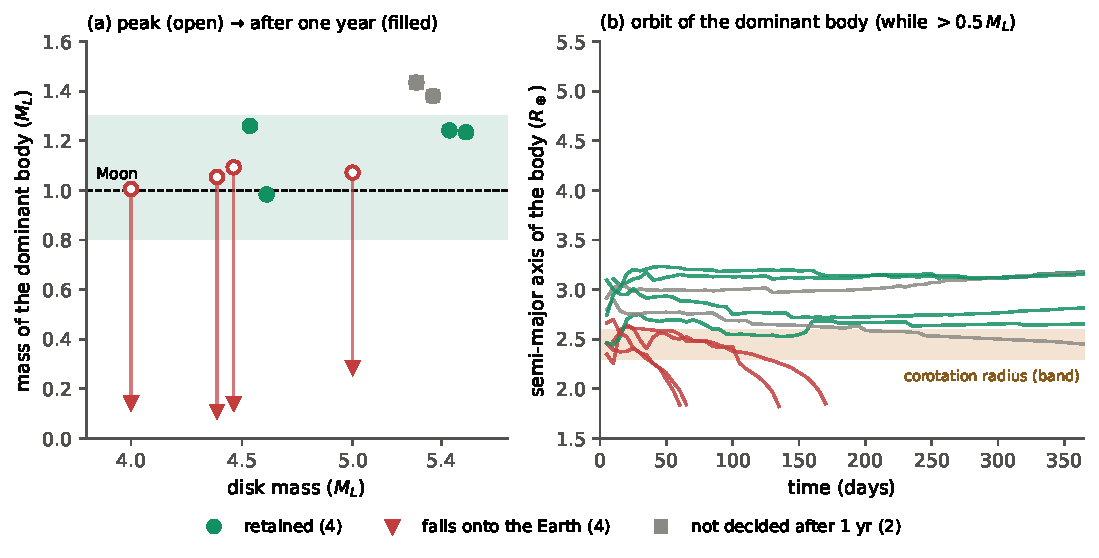
\includegraphics[width=\linewidth]{fig_synth.pdf}
\caption{Synthesis of the ten realizations computed at $6$~h and $1.60\,\Rt$. (a)~Largest mass reached by the dominant body (open circle) and its mass after one year (filled symbol); the gray band is $0.8$--$1.3\,\ML$. (b)~Semi-major axis of the dominant body; the shaded band is the corotation radius. Green: kept. Red: falls onto the Earth between day $65$ and day $175$. Gray: undecided after one year.\label{fig:synth}}
\end{figure}

The criterion adopted is simple. A realization is a success if it forms a body of $0.8$ to $1.3$ lunar masses, whose lowest orbital point stays beyond the corotation radius, on an almost circular orbit whose inclination decreases, and which the tides then bring to $54$--$66\,\Rt$ in $4.5$ billion years. Four realizations satisfy the first two conditions after one year: two at $4.5$ and two at $5.4$ lunar masses. They keep their satellite for five years, from $1.0$ to $1.27$ lunar masses, with nothing falling onto the Earth after the first year. The four realizations that lose the body see it fall between day $65$ and day $175$ (Table~\ref{tab:M45}). Two are undecided after one year.

\begin{table}[htbp]
\centering
\caption{The ten realizations at $6$~h and $1.60\,\Rt$. Peak: largest mass reached by the dominant body; $M_1$, $a_1$: its mass (lunar masses) and semi-major axis ($\Rt$) at the end of the follow-up (one year, or five years for the kept realizations).\label{tab:M45}}
\small
\begin{tabular}{ccccc>{\raggedright\arraybackslash}p{6.0cm}}
\toprule
Disk ($\ML$) & seed & Peak & $M_1$ & $a_1$ & Outcome \\
\midrule
4.0 & 3 & 1.01 & 0.14 & --- & falls onto the Earth (day 170) \\
4.5 & 0 & 1.05 & 0.11 & --- & falls onto the Earth (day 65) \\
4.5 & 1 & 1.09 & 0.14 & --- & falls onto the Earth (day 135) \\
4.5 & 2 & 1.26 & 1.273 & 3.70 & \textbf{kept} over 5 years \\
4.5 & 3 & 0.98 & 1.016 & 3.87 & \textbf{kept} over 5 years \\
5.0 & 3 & 1.07 & 0.29 & --- & falls onto the Earth (day 60) \\
5.4 & 0 & 1.43 & 1.43 & 3.17 & undecided at one year ($a_1>R_{\rm co}$) \\
5.4 & 1 & 1.38 & 1.38 & 2.45 & below the corotation radius, undecided \\
5.4 & 2 & 1.24 & 1.250 & 3.88 & \textbf{kept} over 5 years \\
5.4 & 3 & 1.23 & 1.234 & 4.00 & \textbf{kept} over 5 years \\
\bottomrule
\end{tabular}
\end{table}

\textbf{To retain.} Several disk masses between $4.5$ and $5.4$ lunar masses have given a kept satellite, in about one realization out of two. The favorable interval is not yet delimited: the single calculations at $4.0$ and $5.0$ did not reach a kept satellite, which does not exclude one with other seeds. The value of $4.5$ lunar masses serves as the working value for what follows because one of its realizations ends with a satellite of $1.016$ lunar mass. This is a property of this realization, not of the mass of the disk.

\textbf{Does the body hold near the Roche limit?} The dominant body sits a few Earth radii away, closer than the Roche limit of a liquid ($2.90\,\Rt$). But this limit holds for a liquid. A rubble pile or a paste holds together by its own weight and its contacts. The body is modeled as a pile of $300$ balls that repel on contact and attract at a distance, and one looks at whether it stays in one piece after $20$ revolutions. On the two orbits from phase~C, the pile stays in one piece. The test can nevertheless detect destruction: it tears the pile apart at $1.6$ and $2.0\,\Rt$ and its break-up limit lies between $2.25$ and $2.5\,\Rt$, well below the fluid limit and above that of a rigid solid ($1.49\,\Rt$). The orbits tested stay beyond it, with a margin of $4\,\%$ for the closest.

\subsection{A passage more favorable to braking}
\label{sec:best}

Among the $80$ geometries whose closest point is above the disk, the one that brakes the rotation best is a more grazing and faster passage: $2.6\,\Rt$ and $3$~km\,s$^{-1}$, still retrograde at $25^\circ$. We followed it to the end, with the same code as the reference passage. Table~\ref{tab:bestB} shows that it redistributes a little less material around the Earth ($41\,\%$ stay bound instead of $47\,\%$) without changing the inclination of the orbits ($32^\circ$). The stronger braking therefore costs a little redistribution, without suppressing it.

\begin{table}[htbp]
\centering
\caption{Fate of the tracers for the reference passage and for the passage favorable to braking (computed, average over three seeds, $\Req=1.60\,\Rt$).\label{tab:bestB}}
\small
\begin{tabular}{lcccc}
\toprule
Passage & fallen onto the Earth & bound to the Earth & left the Earth & inclination \\
\midrule
Reference ($3.0\,\Rt$, $2$~km\,s$^{-1}$) & 0.210 & 0.466 & 0.325 & $31.5^\circ$ \\
Favorable ($2.6\,\Rt$, $3$~km\,s$^{-1}$) & 0.265 & 0.410 & 0.325 & $31.9^\circ$ \\
\bottomrule
\end{tabular}
\end{table}

Phase~C is then redone with an Earth rotating in $7.7$~h at the start, the rotation that a removal of $0.21\,\LEM$ would leave. In each of the five realizations completed, a body of $0.71$ to $1.02$ lunar masses forms between days $60$ and $230$; none keeps it at one year. With five realizations against two retentions out of five for the reference passage, the difference is not measurable: this small sample allows us to affirm neither that this passage retains less, nor that it retains as much. Tracking the origin of the particles shows that the dominant body is made of disk material, and the final angular momentum merely repeats that of the start: the dynamics that follow the flyby remove almost nothing. A removal of $0.21\,\LEM$ by the flyby alone is moreover out of reach of a proto-Earth as condensed as this one (Section~\ref{sec:despin}); this $7.7$~h calculation is therefore an extreme test, and the more modest removals of $0.04$ to $0.07\,\LEM$ of the coupled budget have not been tested in phase~C.

\subsection{The tides carry the body to the lunar distance}
\label{sec:migration}

The Earth rotates faster than the body orbits: the tide it raises leads the body, pulls it forward and pushes it outwards, transferring to it angular momentum taken from the rotation of the Earth. The body leaves the Roche limit in less than a year and then moves away without stopping (Table~\ref{tab:migration}, Figure~\ref{fig:migration}). It never reaches synchronism with the rotation of the Earth, and no case falls back.

\begin{table}[htbp]
\centering
\caption{Orbital radius ($\Rt$) of the dominant body from the secular integration of the tides, with a contracting Earth ($\tau_c=10^5$~yr). In parentheses: rotation period of the Earth in hours. The last column gives the radius at $4.5$~Gyr if the dissipation is divided or multiplied by $2$.\label{tab:migration}}
\footnotesize
\begin{tabular}{lcccccc}
\toprule
Kept satellite & $10^3$ yr & $10^6$ yr & $0.25$ Gyr & $1$ Gyr & $4.5$ Gyr & $4.5$ Gyr, dissip. $\times(0.5$--$2)$ \\
\midrule
$1.016\,\ML$ & 8.7 (6.5) & 19.6 (5.5) & 41.9 (7.8) & 50.8 (9.1) & \textbf{62.4} (11.2) & 57--68 \\
$1.273\,\ML$ & 8.9 (6.9) & 19.9 (6.2) & 41.6 (10.7) & 50.0 (13.6) & \textbf{60.2} (19.9) & 55--65 \\
\bottomrule
\end{tabular}
\end{table}

\begin{figure}[htbp]
\centering
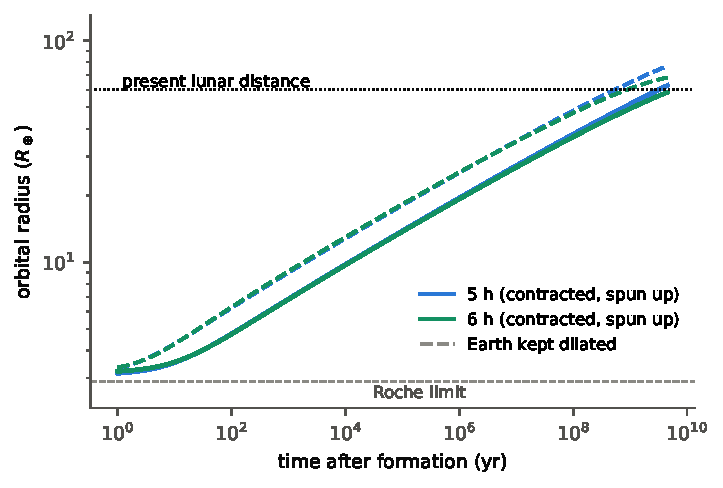
\includegraphics[width=0.82\linewidth]{fig_migration.pdf}
\caption{Orbital radius of the dominant body under the effect of the tides. Solid line: the Earth contracts from the start and its rotation speeds up by conservation of angular momentum. Dashed: the Earth stays swollen. Dotted: present lunar distance; gray dashed: Roche limit.\label{fig:migration}}
\end{figure}

\textbf{To retain.} The two satellites kept at $4.5$ lunar masses reach $62.4$ and $60.2\,\Rt$ in $4.5$ billion years, for a present lunar distance of $60.3\,\Rt$. The agreement is obtained without adjustment, with a dissipation calibrated elsewhere, and it is robust: the distance varies slowly with the dissipation. It does not prove that the Moon followed this path, however; the real dissipation of the Earth has varied over time. The final rotation of the Earth ($11$ to $20$~h instead of $24$~h) is the trace of the excess of angular momentum, which the next section treats. If the Earth contracts as it cools, its rotation speeds up to $3.6$--$4.0$~h, the fast rotation that impact models have to postulate \citep{CukStewart2012}, obtained here without an impact.

% =====================================================================
\section{The angular momentum of the Earth--Moon system}
\label{sec:AM}

Angular momentum measures the ``quantity of rotation'' of a system: that of the Earth spinning on itself and that of the Moon revolving around the Earth. It is conserved: it can pass from the Earth to the Moon through the tides, or be carried away by a body that leaves the system, but it does not disappear. That of the present Earth--Moon system, $\LEM=3.5\times10^{34}$~kg\,m$^2$\,s$^{-1}$, serves as the unit throughout this section. It is the hardest question of all theories of the origin of the Moon, ours included, and it is the one on which this version brings the most that is new.

\subsection{What the Moon says about the rotation of the Earth, read backwards}
\label{sec:obl}

The Moon being a datum, one can integrate the present Earth--Moon system backwards to the epoch when the satellite was at $3.87\,\Rt$, where the flyby leaves it. One obtains what the Earth must then have had as rotation and axial tilt. The result is a \emph{necessary} condition, not an event: other histories lead to the same present. The calculation includes the coupling between the lunar orbit and the equatorial bulge of the Earth, the action of the Sun, and the tides of the Moon and of the Sun.

Three results stand out (Table~\ref{tab:retro}). First, the rotation of the Earth had to carry $0.79\,\LEM$ and the lunar orbit $0.21\,\LEM$, that is $0.994\,\LEM$ in total, whatever the tidal strength assumed; this corresponds to a period of about $7$~h. Second, the obliquity (the angle of the rotation axis with the normal to the ecliptic) had to be $7$ to $13^\circ$. Third, the orbit of the satellite had to be inclined by about $15^\circ$ to the equator, a remarkably stable figure from one case to another.

\begin{table}[htbp]
\centering
\caption{What the Moon requires, read backwards at $3.87\,\Rt$ (computed). $F$: factor by which the tide is multiplied to shorten the calculation; $\varphi$: phase of the node of the lunar orbit, unknown; $\varepsilon_0$: obliquity; $i_{\rm eq}$: inclination of the orbit to the equator.\label{tab:retro}}
\small
\begin{tabular}{lcccc}
\toprule
Case & $\varphi$ ($^\circ$) & $\varepsilon_0$ ($^\circ$) & $i_{\rm eq}$ ($^\circ$) & Rotation of the Earth \\
\midrule
$F=10$ & 0, 90, 180, 270 & 7.3; 10.7; 12.9; 10.6 & 15.1 to 15.5 & $0.79\,\LEM$ \\
$F=4$ & 90, 180 & 6.8; 7.6 & 15.3 to 15.4 & $0.79\,\LEM$ \\
$F=25$ & 90, 180 & 13.1; 10.5 & 15.6 & $0.79\,\LEM$ \\
\bottomrule
\end{tabular}
\end{table}

The same model, integrated this time forwards from the satellite, answers the opposite question: what becomes of a given initial obliquity after $4.5$ billion years (Table~\ref{tab:obl})? The obliquity grows during the evolution, by a factor close to $2.4$ for the first satellite and $1.4$ to $2.3$ for the second. The present $23.4^\circ$ is reached for an initial obliquity of $10$ to $14^\circ$, which agrees with the $7$ to $13^\circ$ of the backward integration. An Earth starting from $0^\circ$ would end below $2.3^\circ$: in this model, a present obliquity of $23^\circ$ cannot come from a primitive obliquity of only a few degrees. The Sun is the essential ingredient: without it, the final obliquity would be about half as large and the lunar orbit would remain inclined by $10$ to $32^\circ$ to the ecliptic instead of less than $4^\circ$.

\begin{table}[htbp]
\centering
\caption{Final obliquity after $4.5$~Gyr as a function of the initial obliquity $\varepsilon_0$ (computed). The range covers two phases of the node of the lunar orbit.\label{tab:obl}}
\small
\begin{tabular}{rcc}
\toprule
$\varepsilon_0$ ($^\circ$) & satellite of $1.273\,\ML$ & satellite of $1.016\,\ML$ \\
\midrule
0 & 0.4 & 2.3 \\
5 & 12.0--12.7 & 7.0--11.5 \\
10 & 24.0--24.7 & 16.2--20.6 \\
15 & 35.3--35.9 & 25.2--29.4 \\
20 & 45.7--46.4 & 33.9--38.0 \\
\bottomrule
\end{tabular}
\end{table}

\textbf{To retain.} Read backwards, the Moon asks for an Earth rotating in about $7$~h with a slightly inclined axis, at the moment when the flyby leaves the satellite at $3.9\,\Rt$. The planets were examined by a comparison of speeds along the backward path: the precession of the axis stays at least $1.9$ times faster than the largest planetary frequency, so that their influence is probably weak, with a reservation from the literature about a resonance island for a fast-rotating Earth \citep{LaskarJoutelRobutel1993}. The model has neither planets nor eccentricity.

\textbf{The other planets as a point of reference.} The orbits of the planets are all close to the ecliptic (less than $7.1^\circ$), but their rotation axes range from $0.01^\circ$ to $178^\circ$: the Sun does not orient the axis of a planet towards its orbit. For the four inner planets, \citet{LaskarRobutel1993} conclude that none of the obliquities can be considered primordial, whereas the four giant planets have kept theirs since their formation. Random initial axes are therefore the rule, and the axis of the proto-Earth before the flyby, which the theory does not constrain, is nothing exceptional.

\subsection{The excess of $0.21\,\LEM$}
\label{sec:excess}

The bound system that the calculation produces is the following (Table~\ref{tab:AM45}). For the satellite of $1.016$ lunar mass, the rotation of the Earth, including the angular momentum of the bodies that fell onto it, carries $0.996\,\LEM$ and the whole bound system, orbit included, $1.208\,\LEM$. The present Earth--Moon system, scaled to a satellite of the same mass, carries $0.999\,\LEM$. The bound system therefore holds $0.21\,\LEM$ too much. The small bodies that left the system carried away only $0.017$ of it, already counted. For the satellite of $1.273$ lunar mass, too massive by $27\,\%$ relative to the Moon, the excess is only $0.04\,\LEM$, but only because a heavier satellite requires more orbital angular momentum at the same distance; this does not make it a better match.

\begin{table}[htbp]
\centering
\caption{Angular-momentum budget of the two satellites kept at $4.5$ lunar masses, in units of $\LEM$ (computed). The ``required'' value is that of an Earth--Moon system with the same satellite mass, at $60.3\,\Rt$, with a $24$~h Earth.\label{tab:AM45}}
\small
\begin{tabular}{lcc}
\toprule
Item & satellite of $1.016\,\ML$ & satellite of $1.273\,\ML$ \\
\midrule
Rotation of the Earth at five years & 0.996 & 0.985 \\
Bound system, total & 1.208 & 1.249 \\
Carried away by the bodies that left the system & 0.017 & 0.018 \\
Required by the present system & 0.999 & 1.209 \\
\textbf{Excess} & \textbf{0.21} & \textbf{0.04} \\
Rotation of the Earth at $4.5$~Gyr, lunar tide alone & 11.2 h & 19.9 h \\
\bottomrule
\end{tabular}
\end{table}

\textbf{How to place this excess.} It is of the same order as the bound of $1.2\,\LEM$ that \citet{Canup2014} retains for ``canonical'' impacts, and four to nine times smaller than that of high-angular-momentum impacts, whose total is $1.9$ to $2.8\,\LEM$ (that is, $0.9$ to $1.8\,\LEM$ of excess) and which the evection must then remove. Fast-Earth variants must also evacuate angular momentum \citep{CukStewart2012,Tremaine2009}. Our excess depends on the starting state: the $6$~h rotation and the moment of inertia of the swollen Earth ($0.187\,\Mt\Req^2$). A faster rotation or a more condensed body would carry more.

\begin{table}[htbp]
\centering
\caption{Total angular momentum and excess for three families of pathways, in units of $\LEM$. The impact values come from \citet{Canup2014}; that of this study is computed here (realization of $1.016\,\ML$).\label{tab:compAM}}
\small
\begin{tabular}{lcc}
\toprule
Pathway & Total & Excess over $1\,\LEM$ \\
\midrule
Canonical impact (bound) & up to $1.2$ & up to $0.2$ \\
High-angular-momentum impacts & $1.9$ to $2.8$ & $0.9$ to $1.8$ \\
This study, before the removal mechanisms & $1.21$ & $0.21$ \\
\bottomrule
\end{tabular}
\end{table}

\subsection{What planet~$B$ removes from the rotation}
\label{sec:despin}

Planet~$B$ does not leave empty-handed. In passing, it raises a tidal bulge on the proto-Earth. This bulge lags behind the direction of planet~$B$ because the material does not respond instantaneously; the attraction of planet~$B$ on this offset bulge brakes the rotation of the Earth, the corresponding heat is dissipated in the Earth, and the angular momentum lost by the rotation passes into the motion of planet~$B$. The flyby being retrograde, the surface of the Earth runs under planet~$B$ at the relative speed $\Omega_\oplus+|\dot\phi_B|$, always positive: \emph{the sign of the braking is therefore certain}. Its size depends on the amount of tide that the Earth turns into heat.

\textbf{A soft body, neither liquid nor rigid.} A liquid follows the tide without friction; a cold solid hardly deforms; the dissipation is strongest between the two, for a soft material. This is the case of the proto-Earth of this theory, and the passage of planet~$B$ does not change this character. We computed how far this dissipation goes with a Maxwell rheology, which describes a material that is elastic for fast tides and viscous for slow tides, first for a uniform body, then for stratified bodies (a liquid core, a pasty mantle, a swollen envelope). Three results stand out.

\begin{enumerate}[leftmargin=1.6em,itemsep=2pt]
\item \emph{The material that dissipates best is a thick paste}, of viscosity of the order of $10^{12}$~Pa\,s (about a million billion times that of water), not a liquid. A liquid envelope dissipates almost nothing. The dissipation must therefore take place in the soft material, through the whole thickness of the body.
\item \emph{The fact that the tide rises and then falls during the flyby does not change the result}: a calculation that follows the tide instant by instant gives the same braking to within $2\,\%$, because the effect concentrates around the closest point and the paste reacts within minutes.
\item \emph{The maximum dissipation depends on the condensation of the body.} The more condensed the Earth is towards the center, the less it deforms and the less it dissipates (Table~\ref{tab:interieur}).
\end{enumerate}

The maximum dissipation of a uniform body grows with its rigidity up to a plateau (Table~\ref{tab:rigidite}). It is almost zero for a nearly liquid body ($0.013$ for $0.1$~GPa), reaches $0.26$ near $3$~GPa, which suffices for the favorable passage, and $0.48$ at $10$~GPa, which suffices for both passages. A material with some rigidity is therefore needed, that is, a paste and not a liquid.

\begin{table}[htbp]
\centering
\caption{Maximum dissipation $k_2/Q$ of a uniform body of Maxwell rheology, as a function of its rigidity (computed, most favorable viscosity).\label{tab:rigidite}}
\small
\begin{tabular}{cccccc}
\toprule
Rigidity (GPa) & $0.1$ & $1$ & $3$ & $10$ & $70$ \\
\midrule
maximum $k_2/Q$ & 0.013 & 0.115 & 0.263 & 0.483 & 0.695 \\
\bottomrule
\end{tabular}
\end{table}

\begin{table}[htbp]
\centering
\caption{Maximum braking that Maxwell rheology allows, in $\LEM$, for a few stratified bodies whose reduced moment of inertia $C/(MR^2)$ varies (computed). ``Reference passage'': distance $3.0\,\Rt$, $2$~km\,s$^{-1}$. ``Favorable passage'': $2.6\,\Rt$, $3$~km\,s$^{-1}$. The monograph uses $C/(MR^2)=0.187$ for the swollen proto-Earth.\label{tab:interieur}}
\small
\begin{tabular}{lccc}
\toprule
Body & $C/(MR^2)$ & reference passage & favorable passage \\
\midrule
Core and mantle, without envelope & 0.30 & 0.21 & 0.38 \\
Envelope of $0.22$ Earth mass & 0.20 & 0.05 & 0.09 \\
Envelope of $0.17$ (monograph value) & 0.19 & \textbf{0.04} & \textbf{0.07} \\
Envelope of $0.50$ & 0.29 & 0.18 & 0.33 \\
\bottomrule
\end{tabular}
\end{table}

\textbf{To retain.} For a proto-Earth as condensed as in this study, a soft body removes at most $0.04\,\LEM$ with the reference passage and $0.07\,\LEM$ with the most favorable passage; with the tide used in the monograph, the removal is more modest still, $0.012$ to $0.027\,\LEM$. It is therefore \emph{not} the only mechanism able to close the budget; it is a real contribution, of the order of $0.01$ to $0.07\,\LEM$ depending on the dissipation of the soft material. A markedly less condensed body would remove more, but it would also carry more angular momentum at equal period, and this second case has not been recomputed.

\textbf{The axis.} The same flyby tilts the axis of the Earth without changing the angular momentum of the rotation. The tilt depends on the flattening of the proto-Earth, which is not known for a hot body: it ranges from $2^\circ$ to $30^\circ$ according to this flattening. The interval of $7$ to $13^\circ$ that the Moon asks for lies within this range, which is a consistency of orders of magnitude and not a test. The axis does not become parallel to the orbit of planet~$B$. One gap remains unresolved: the flattening that gives a tilt of $10^\circ$ is not that of the stratified body closest to the monograph, and a single interior model that would give together moment of inertia, flattening, dissipation and rotation is not built.

\subsection{The other mechanisms, taken one by one}
\label{sec:puits}

Three other mechanisms remove angular momentum, which we first tested separately.

\textbf{The solar tide on the Earth.} The Sun also raises a tide on the Earth, which brakes its rotation, the angular momentum lost passing to the orbit of the Earth around the Sun. With the same dissipation as the lunar tide, it removes $0.017\,\LEM$ in $4.5$ billion years, about $8\,\%$ of the excess.

\textbf{Bodies that leave the system.} The small unbound bodies carry away $0.017$ to $0.018\,\LEM$. They are already counted in the budget of Table~\ref{tab:AM45}.

\textbf{The evection resonance.} When the satellite is still close to the Earth, the precession of its orbit can synchronize with the period of revolution of the Earth around the Sun. The satellite is then trapped for a time in a resonance where its orbit lengthens strongly; during this trapping, the gravity of the Sun takes angular momentum from the Earth--Moon system for the benefit of the orbit of the Earth around the Sun, and the system comes out lighter \citep{CukStewart2012,WardCanupRufu2020,RufuCanup2020}. We studied it with a planar secular model (Appendix~\ref{app:evec}). With a terrestrial tide of at least $0.1$ times the reference, it removes at most $0.03\,\LEM$; larger values, up to $0.06\,\LEM$, are obtained only with tides $100$ to $1000$ times weaker, which would leave the satellite at only about twenty Earth radii after $4.5$ billion years. These values are those of the mechanism taken in isolation; the contraction time of the proto-Earth, which controls the yield, enters only in the coupled budget (Section~\ref{sec:couple}), where the mean removal reaches $0.16\,\LEM$ for $\tau_c=2\times10^6$~yr, and the duration of the captures is given in Appendix~\ref{app:trois}.

\textbf{To retain.} Taken separately, none of these mechanisms removes $0.21\,\LEM$. The solar tide removes $0.017$, the braking by planet~$B$ $0.01$ to $0.07$, the evection up to $0.03$ for a usual terrestrial tide. But they do not simply add up, because they act on the same system, one after the other, and each modifies the conditions of the next. The budget must therefore be computed on a single trajectory.

\subsection{The mechanisms act together: the coupled budget}
\label{sec:couple}

The three mechanisms follow one another in time and modify one another. The braking by planet~$B$ takes place in a few hours, and it fixes the rotation with which the Earth enters what follows. The evection is played out afterwards over thousands to millions of years, as long as the satellite is close; it depends on the rotation of the Earth, on its tide and on its radius, which decreases while the proto-Earth cools. The lunar tide and the solar tide finish the work over billions of years. The removals computed separately therefore cannot be added. We built a calculation that chains the three stages on \emph{a single trajectory}, starting from the kept satellite of $1.016$ lunar mass.

\textbf{The precisions that fix the framework.} Three points, which are choices of the theory, determine this calculation.
\begin{itemize}[leftmargin=1.6em,itemsep=2pt]
\item The proto-Earth is a body that is \emph{soft, never liquid}. The passage of planet~$B$ changes nothing of this character.
\item Planet~$B$ nevertheless carries away a little rotational angular momentum, as seen in Section~\ref{sec:despin}. We represent it by a removal $\Delta L_B$, taken as $0$, $0.04$ or $0.07\,\LEM$ (and from $0.05$ to $0.20\,\LEM$ in a first scan). The values $0.04$ and $0.07$ are the maximum that a soft body as condensed as in this study allows, for the reference passage and for the most favorable passage.
\item The tide of a soft body is not that of a solid body, which explains a weakness at the beginning of the history. We translate this by an \emph{early} terrestrial tide, during the passage through the evection, equal to a small fraction of the reference tide ($0.03$ to $0.3\,\%$). This weakness is \emph{posed} by the calculation, not demonstrated: the dissipation of a soft body depends on its viscosity, which we have not computed for this phase. It is a condition to be established.
\end{itemize}

\textbf{The calculation.} The starting rotation is that of Section~\ref{sec:excess} reduced by $\Delta L_B$. The proto-Earth contracts from $1.60\,\Rt$ to $1\,\Rt$ with a characteristic time $\tau_c$, which the calculation varies from a hundred thousand to a few million years. The satellite enters the evection resonance, is trapped or not depending on its phase of arrival, then, when it leaves it, the lunar tide and the solar tide carry it to $4.5$ billion years. The tide of the last billions of years is \emph{adjusted} so that the final distance is exactly $60.3\,\Rt$; it is not imposed, since the real dissipation of the Earth has varied over time. The calculation is moreover not made to reproduce the present recession of the Moon ($3.8$~cm per year, against $1.15$ in the model at the end): it transfers rotation to the orbit without removing anything, so that the final excess depends little on this detail. The total angular momentum is conserved to $10^{-6}\,\LEM$ at each stage. Without evection or braking, the calculation recovers the values of Section~\ref{sec:puits} ($1.191\,\LEM$ and $62.2\,\Rt$ with the solar tide alone).

\textbf{What the calculation gives, and how we read it.} The result of each trajectory is the \emph{final excess}: the angular momentum of the system at $4.5$ billion years, minus that which the Moon requires ($0.999\,\LEM$). The target is fixed; only the initial excess to be removed varies from one realization to another.
\[
\Delta L_{\rm final}=L_{\rm computed}-L_{\rm target},
\qquad
\text{budget closed}\iff|\Delta L_{\rm final}|\le\varepsilon .
\]
A zero final excess would be a perfect closure; an excess of $+0.10\,\LEM$ means that the system keeps too much, an excess of $-0.10\,\LEM$ that it has lost too much. No calculation lands exactly on zero, so a tolerance has to be chosen. We call \emph{window} its half-width $\varepsilon$: with $\varepsilon=0.05\,\LEM$, the budget is said to be closed if the final excess lies between $-0.05$ and $+0.05\,\LEM$. An excess that is too negative therefore does not close the budget, even if the mechanism removed enough angular momentum: the trajectory does not reach closure. The same holds for a trajectory in which the Moon is lost.

We do not fix a single window, because none is imposed by the physics of the problem. We give four, from $\pm0.03$ to $\pm0.10\,\LEM$.
\begin{itemize}[leftmargin=1.6em,itemsep=2pt]
\item $\pm0.03\,\LEM$ is a \emph{strict} comparison criterion. It is of the same order as the spread from one trajectory to another, which comes from differences between trajectories of the model (phase of arrival in the resonance, parameters), not necessarily from a computational error.
\item $\pm0.08\,\LEM$ is a \emph{broad exploratory} criterion. It reflects the fact that the initial excess depends on the realization: it is $0.21\,\LEM$ for the one we follow and $0.04\,\LEM$ for another, a difference of $0.17\,\LEM$ whose half is of the order of $0.08\,\LEM$. This is a sensitivity scale between two realizations, not a statistical margin of error; we do not present it as a tolerance deduced from the physics.
\end{itemize}
The results are given as \emph{shares of trajectories} of the parameter grid explored (early tide, lunar dissipation, phase of arrival, contraction time). These shares are not probabilities. With $36$ trajectories per row, one trajectory weighs about $2.8$ percentage points: a difference of one or two grid points has no statistical weight. Four results stand out.

\paragraph{1. The contraction time controls the yield of the evection.} For a proto-Earth that contracts fast ($\tau_c\le2\times10^5$ yr), the evection removes on average only $0.03$ to $0.05\,\LEM$, and the budget closes at $\pm0.03\,\LEM$ in no trajectory without braking by planet~$B$. For a slower contraction, from $3\times10^5$ to $2\times10^6$ yr, it removes on average from $0.04$ to $0.16\,\LEM$ depending on the case, with trajectories that reach $0.30\,\LEM$ (Table~\ref{tab:couple}). The satellite stays kept, except for the longest contractions, where it is lost onto the Earth in part of the trajectories. Capture durations in the grid range from $0.5$ to $435$ thousand years (appendix~\ref{app:trois}); the sensitivity of the closure shares to the evection yield and to the starting state is given in appendix~\ref{app:ferm}.

\begin{table}[htbp]\centering\footnotesize\setlength{\tabcolsep}{3.6pt}
\caption{Coupled budget, trajectory by trajectory: for each removal $\Delta L_B$ by planet~$B$ and each contraction time $\tau_c$ (in yr), mean and maximum removal by the evection, final excess (mean, minimum, maximum), fraction of trajectories whose final excess lies between $-\varepsilon$ and $+\varepsilon$ for four windows, and number of trajectories where the Moon is lost (they do not close the budget). Each row groups $36$ trajectories (three early tides from $0.03$ to $0.3\,\%$, three lunar dissipations, four phases); one trajectory therefore represents about $2.8$ percentage points. Excesses are in units of $\LEM$.\label{tab:couple}}
\begin{tabular}{ccccccccc}\toprule
$\Delta L_B$ & $\tau_c$ & evection mean (max.) & final excess mean [min.\,; max.] & $\varepsilon{=}0.03$ & $0.05$ & $0.08$ & $0.10$ & Moon lost \\
\midrule
0.00 & 100~k & 0.03 (0.12) & 0.16 [0.07\,; 0.19] & 0\,\% & 0\,\% & 3\,\% & 6\,\% & 0/36 \\
0.00 & 200~k & 0.05 (0.14) & 0.15 [0.06\,; 0.19] & 0\,\% & 0\,\% & 14\,\% & 17\,\% & 0/36 \\
0.00 & 300~k & 0.08 (0.20) & 0.11 [0.00\,; 0.19] & 17\,\% & 19\,\% & 33\,\% & 39\,\% & 0/36 \\
0.00 & 500~k & 0.10 (0.25) & 0.09 [$-$0.06\,; 0.19] & 11\,\% & 25\,\% & 44\,\% & 50\,\% & 0/36 \\
0.00 & 1~M & 0.13 (0.30) & 0.06 [$-$0.11\,; 0.19] & 25\,\% & 25\,\% & 39\,\% & 58\,\% & 0/36 \\
0.00 & 2~M & 0.16 (0.29) & 0.03 [$-$0.10\,; 0.19] & 6\,\% & 28\,\% & 50\,\% & 64\,\% & 4/36 \\
\addlinespace
0.04 & 100~k & 0.03 (0.09) & 0.13 [0.06\,; 0.15] & 0\,\% & 0\,\% & 8\,\% & 19\,\% & 0/36 \\
0.04 & 200~k & 0.05 (0.15) & 0.11 [0.00\,; 0.15] & 8\,\% & 14\,\% & 25\,\% & 39\,\% & 0/36 \\
0.04 & 300~k & 0.07 (0.19) & 0.08 [$-$0.03\,; 0.15] & 17\,\% & 31\,\% & 47\,\% & 56\,\% & 0/36 \\
0.04 & 500~k & 0.10 (0.29) & 0.05 [$-$0.14\,; 0.15] & 6\,\% & 31\,\% & 50\,\% & 75\,\% & 0/36 \\
0.04 & 1~M & 0.11 (0.28) & 0.04 [$-$0.12\,; 0.15] & 22\,\% & 25\,\% & 50\,\% & 56\,\% & 2/36 \\
0.04 & 2~M & 0.12 (0.28) & 0.03 [$-$0.13\,; 0.15] & 19\,\% & 22\,\% & 33\,\% & 47\,\% & 6/36 \\
\addlinespace
0.07 & 100~k & 0.02 (0.10) & 0.10 [0.02\,; 0.12] & 3\,\% & 6\,\% & 17\,\% & 33\,\% & 0/36 \\
0.07 & 200~k & 0.05 (0.14) & 0.07 [$-$0.01\,; 0.12] & 22\,\% & 28\,\% & 50\,\% & 56\,\% & 0/36 \\
0.07 & 300~k & 0.04 (0.16) & 0.08 [$-$0.03\,; 0.12] & 8\,\% & 36\,\% & 44\,\% & 56\,\% & 0/36 \\
0.07 & 500~k & 0.08 (0.21) & 0.04 [$-$0.08\,; 0.12] & 22\,\% & 31\,\% & 64\,\% & 69\,\% & 1/36 \\
0.07 & 1~M & 0.10 (0.25) & 0.02 [$-$0.13\,; 0.12] & 8\,\% & 33\,\% & 44\,\% & 50\,\% & 2/36 \\
0.07 & 2~M & 0.09 (0.22) & 0.03 [$-$0.10\,; 0.12] & 19\,\% & 19\,\% & 31\,\% & 31\,\% & 11/36 \\
\bottomrule\end{tabular}\end{table}

\paragraph{2. The budget closes in a notable share of the trajectories, and planet~$B$ helps modestly.} Table~\ref{tab:fenetres} gives the share of trajectories that close the budget, for contractions of $5\times10^5$ to $10^6$ yr and for each window.

\begin{table}[htbp]\centering\small
\caption{Fraction of trajectories that close the budget, according to the window $\varepsilon$ (the budget is closed if the final excess lies between $-\varepsilon$ and $+\varepsilon$, in units of $\LEM$). Contraction times from $5\times10^5$ to $10^6$ yr; each cell groups $36$ trajectories per duration, the range giving the two durations. A lost Moon counts among the trajectories that do not reach closure. These are shares of a parameter grid, not probabilities; the window $\pm0.03$ is a strict comparison criterion, the window $\pm0.08$ a broad exploratory one.\label{tab:fenetres}}
\begin{tabular}{cccc}\toprule
Window $\varepsilon$ & no braking by $B$ & $B$ removes $0.04\,\LEM$ & $B$ removes $0.07\,\LEM$ \\
\midrule
$\pm0.03$ (strict) & 11\,--\,25\,\% & 6\,--\,22\,\% & 8\,--\,22\,\% \\
$\pm0.05$ & 25\,\% & 25\,--\,31\,\% & 31\,--\,33\,\% \\
$\pm0.08$ (broad) & 39\,--\,44\,\% & 50\,\% & 44\,--\,64\,\% \\
$\pm0.10$ & 50\,--\,58\,\% & 56\,--\,75\,\% & 50\,--\,69\,\% \\
\bottomrule\end{tabular}\end{table}

The reading is as follows. At $\pm0.05\,\LEM$, the budget closes in about a quarter to a third of the trajectories ($25$ to $33\,\%$), and at $\pm0.08\,\LEM$ in about two fifths to two thirds ($39$ to $64\,\%$). At the strict criterion of $\pm0.03\,\LEM$, the share is $6$ to $25\,\%$. Braking by planet~$B$ does not improve the share at every window: at $\pm0.03\,\LEM$, the shares with and without braking overlap. It does, on the other hand, increase the share at intermediate and broad windows, above all for the contraction of $5\times10^5$ yr, where the share at $\pm0.08\,\LEM$ goes from $44\,\%$ without braking to $50\,\%$ with $0.04\,\LEM$ and to $64\,\%$ with $0.07\,\LEM$. This is a tendency, at the scale of the grid. Each $0.01\,\LEM$ removed by planet~$B$ is that much less for the evection to remove, which explains the tendency (Figures~\ref{fig:etapes}, \ref{fig:tauc} and~\ref{fig:carte}).

A neighboring quantity must not be confused with closure: in $25$ to $47\,\%$ of the trajectories of these durations, the mechanism removes \emph{at least} the required level (final excess less than or equal to $+0.03\,\LEM$, whatever its negative value). This is a measure of removal capacity, which also counts the trajectories that remove too much. For the longest contractions, the satellite is lost onto the Earth in part of the trajectories ($11$ out of $36$ at $2\times10^6$ yr with $0.07\,\LEM$): these trajectories do not reach closure, which bounds the window from above.

\begin{figure}[htbp]
\centering
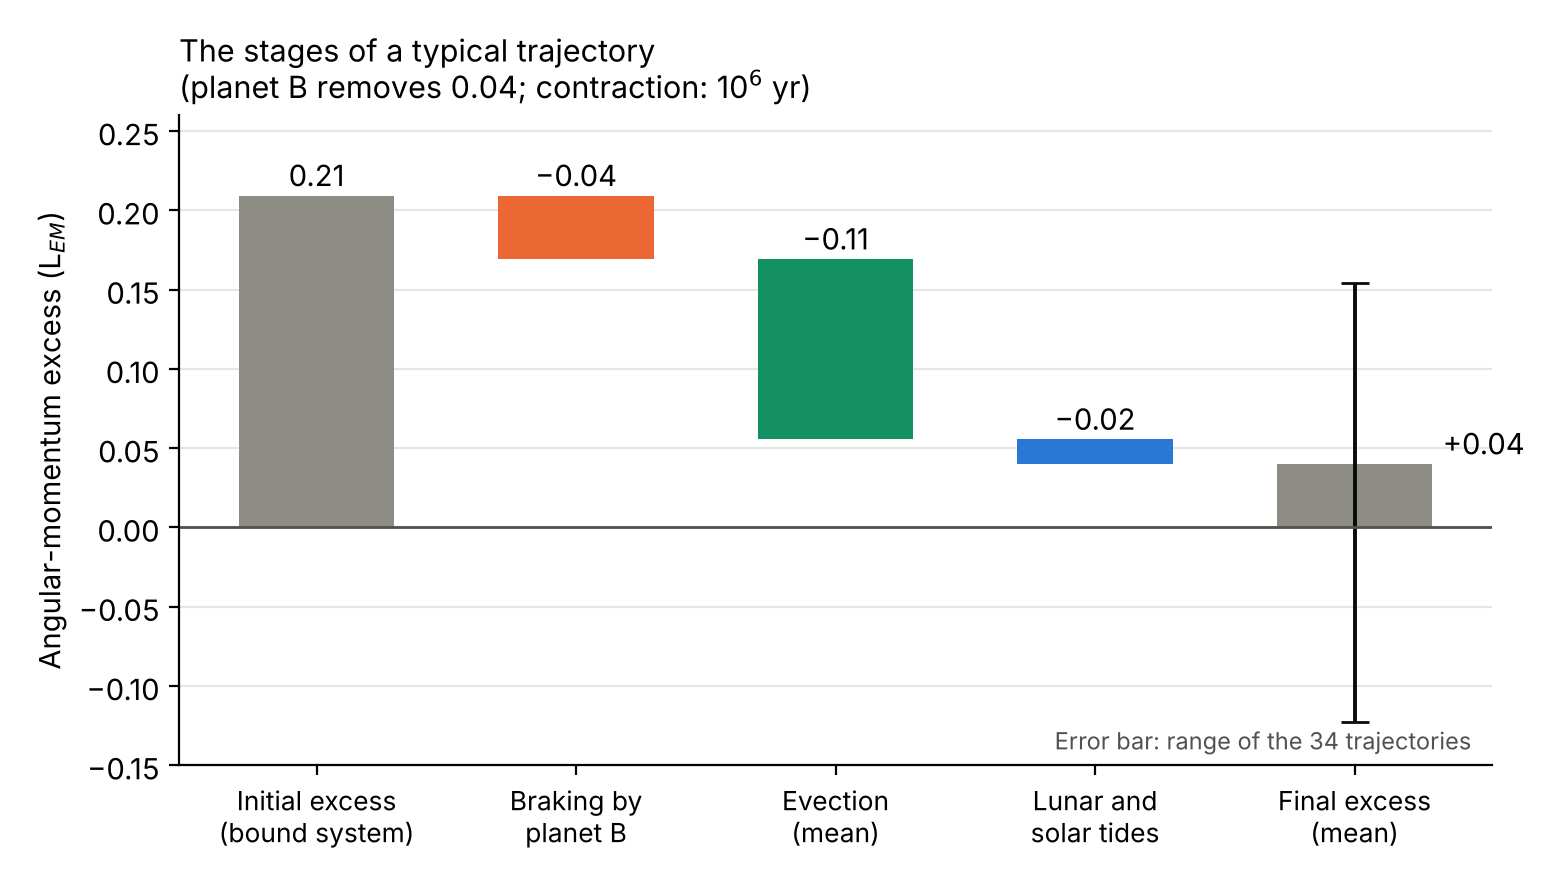
\includegraphics[width=0.78\linewidth]{fig_etapes_en.png}
\caption{The stages of a typical trajectory, averaged over the $34$ trajectories where the satellite is kept (removal of $0.04\,\LEM$ by planet~$B$, contraction of $10^6$ yr): the initial excess of $0.21\,\LEM$ is reduced by the braking by planet~$B$, by the evection, then by the tides. The error bar gives the range of the final excess, from $-0.12$ to $+0.15\,\LEM$.\label{fig:etapes}}
\end{figure}

\begin{figure}[htbp]
\centering
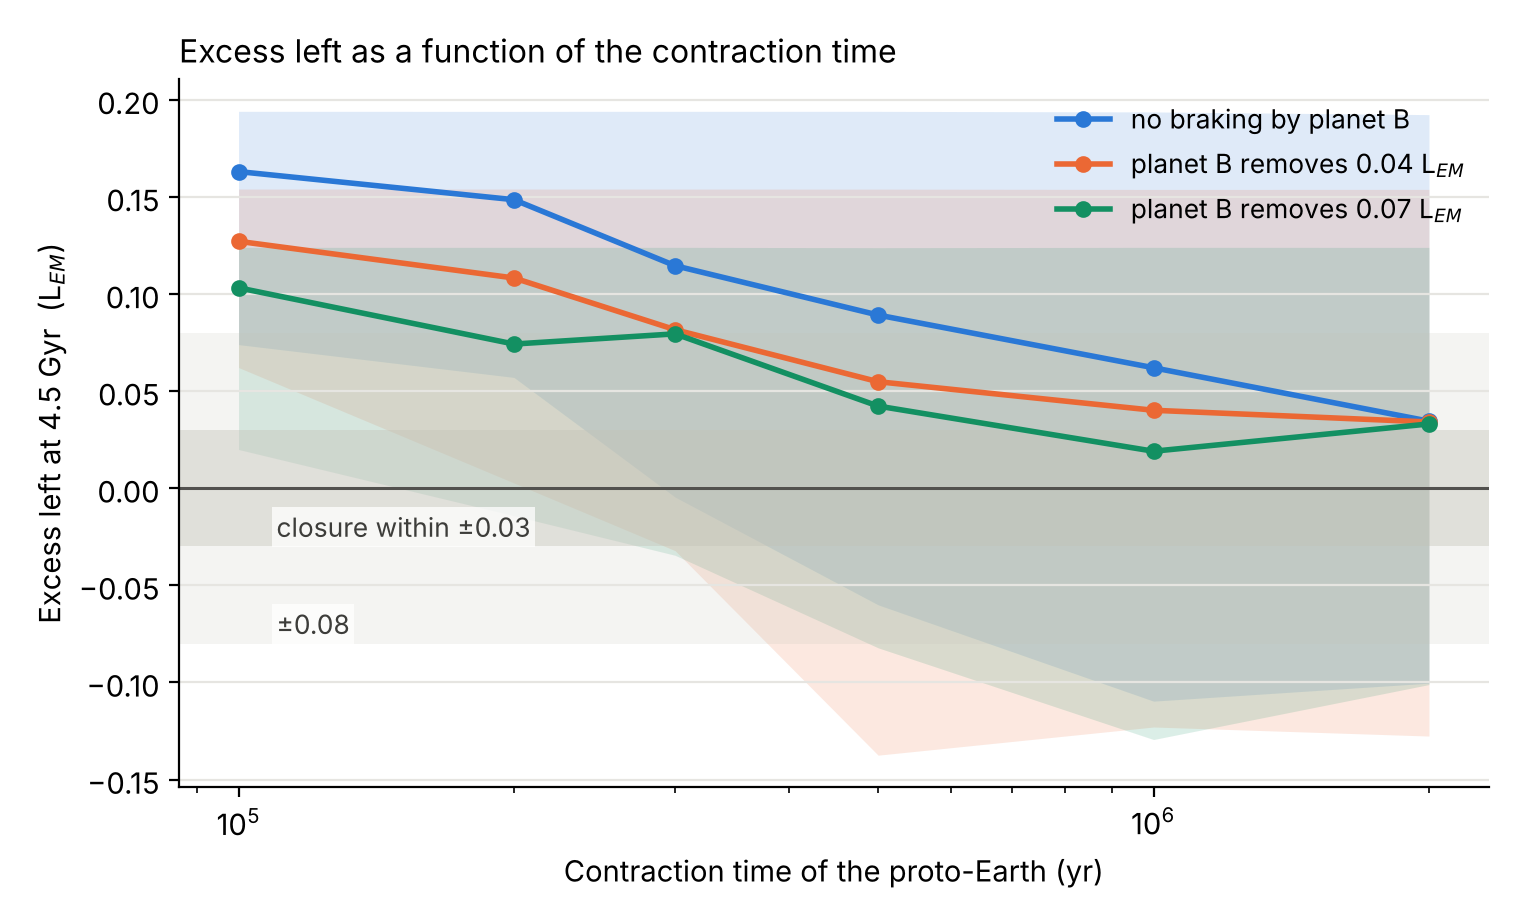
\includegraphics[width=0.78\linewidth]{fig_tauc_en.png}
\caption{Angular-momentum excess left at $4.5$ billion years, as a function of the contraction time of the proto-Earth. The line is the mean, the colored zone the range of the trajectories; the dark gray band is the strict window ($\pm0.03\,\LEM$), the light band the broad exploratory window ($\pm0.08\,\LEM$). A negative excess means that the trajectory removed more than necessary.\label{fig:tauc}}
\end{figure}

\begin{figure}[htbp]
\centering
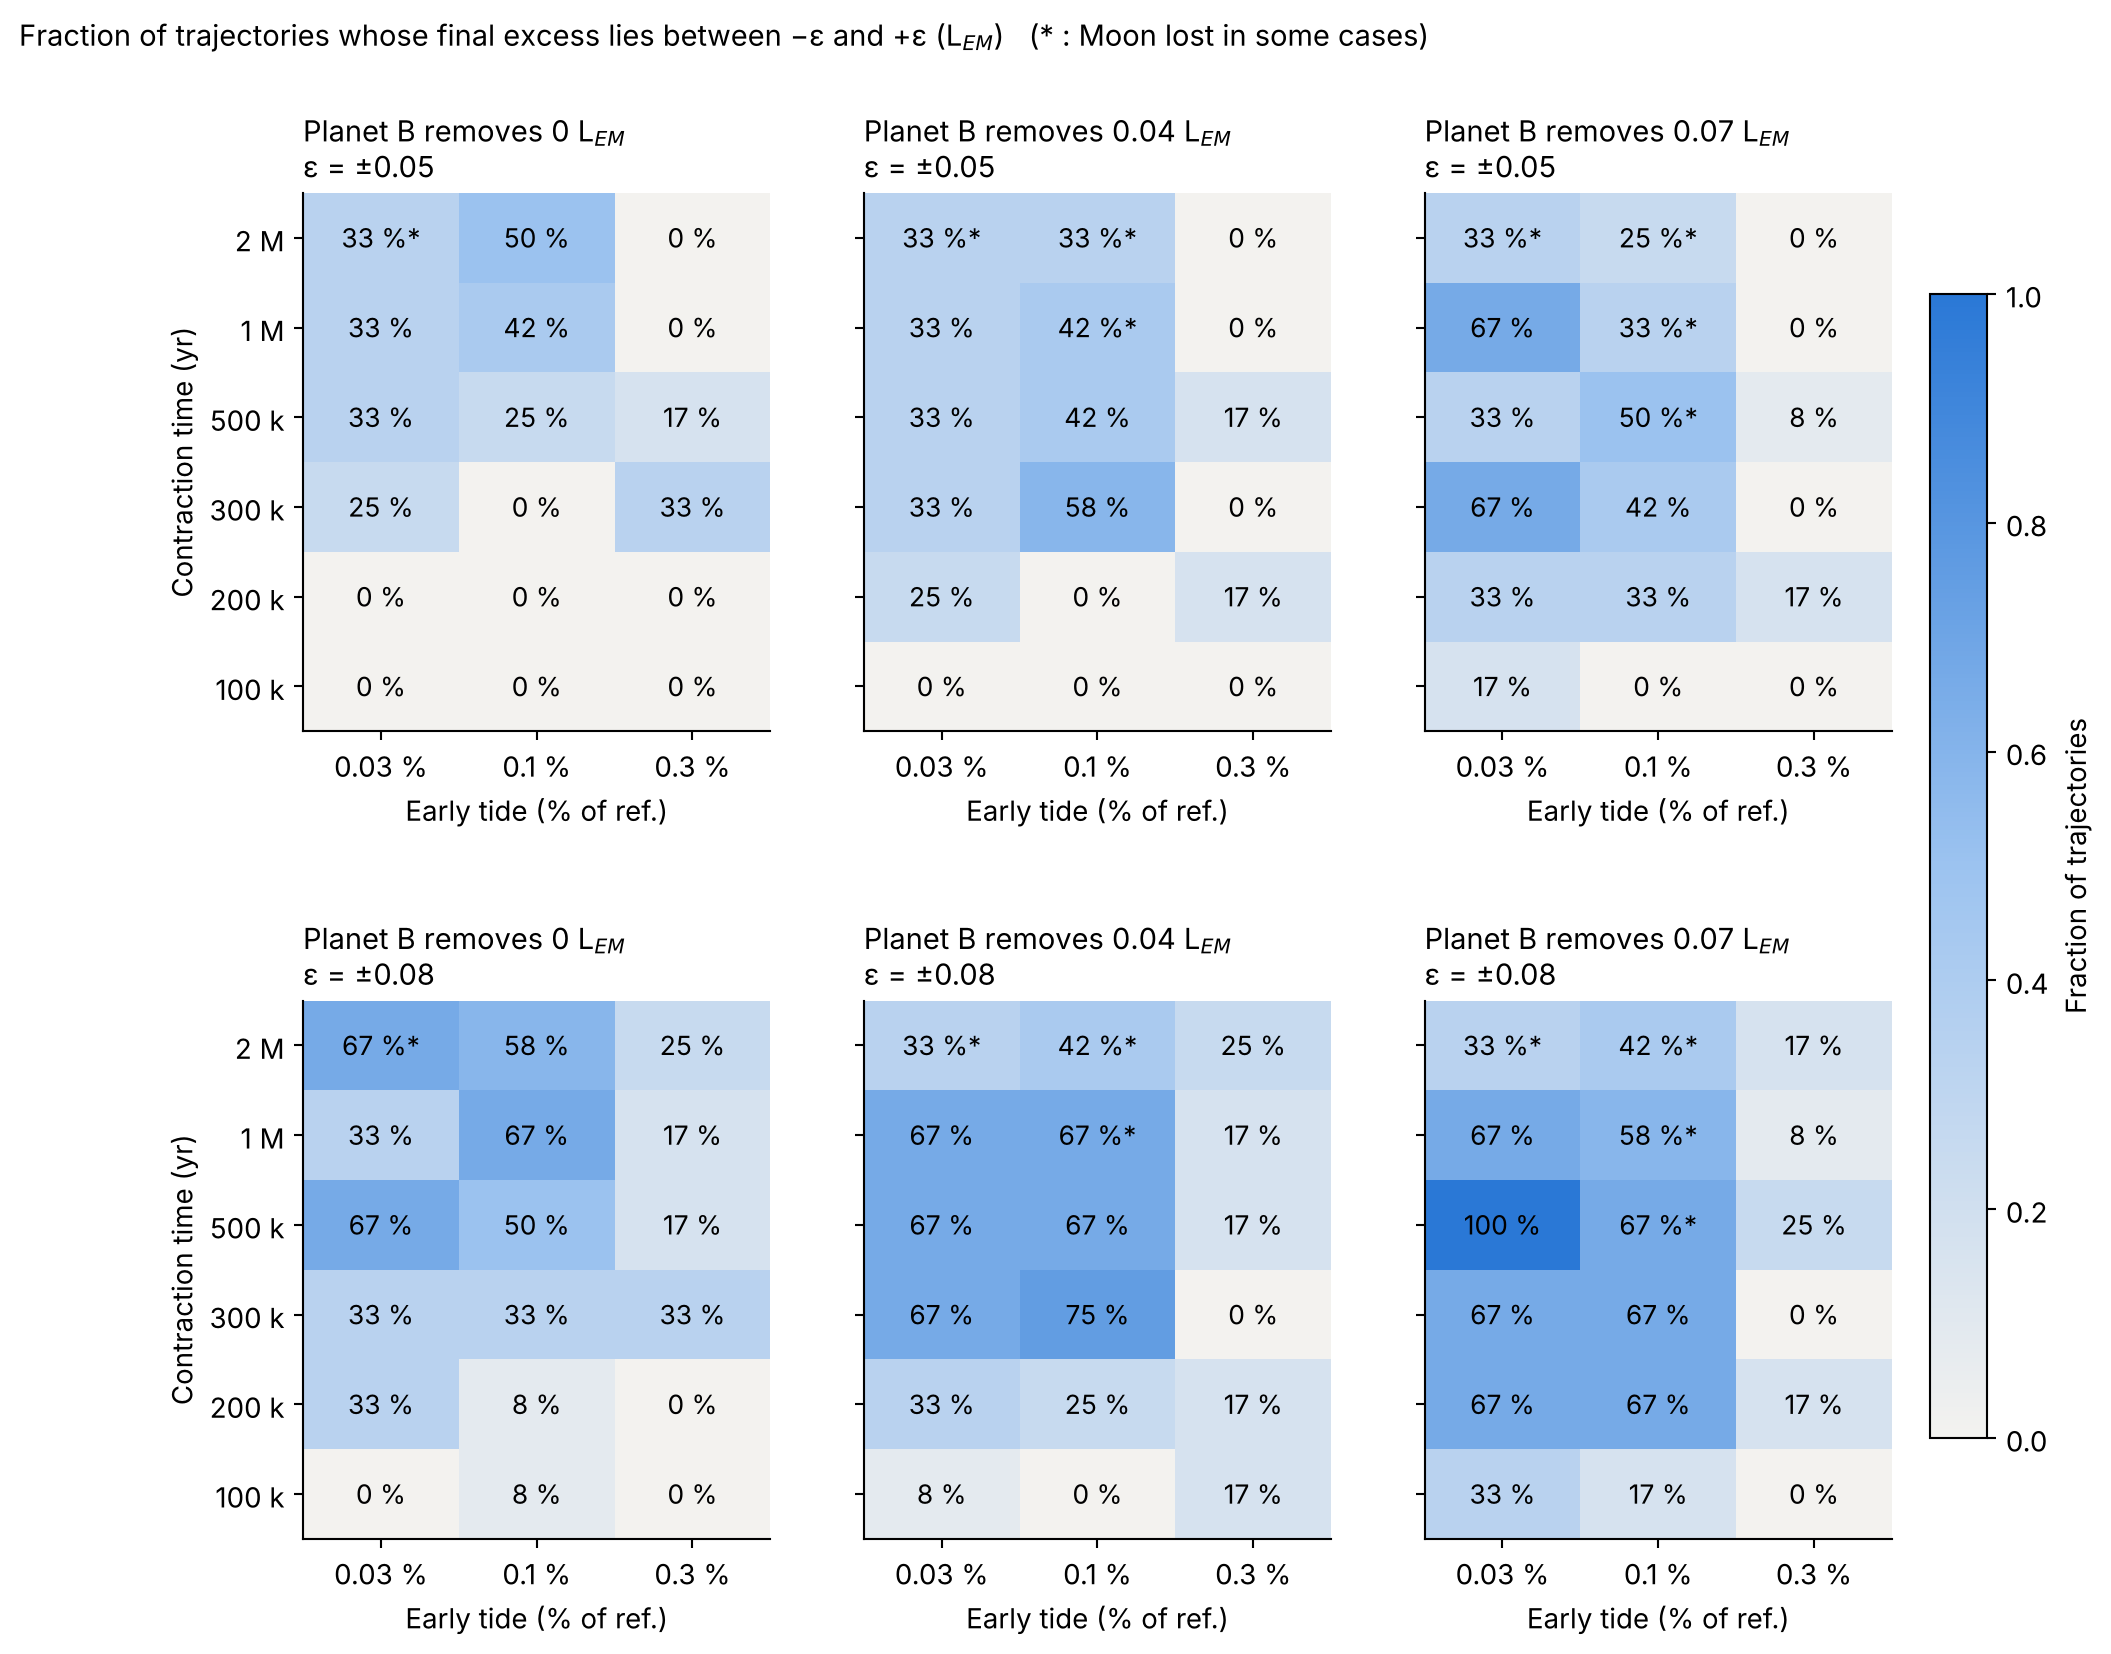
\includegraphics[width=\linewidth]{fig_map_en.png}
\caption{Fraction of the trajectories whose final excess lies between $-\varepsilon$ and $+\varepsilon$, for $\varepsilon=0.05\,\LEM$ (top) and $0.08\,\LEM$ (bottom), as a function of the contraction time of the proto-Earth and of the early terrestrial tide, for three values of the removal by planet~$B$. Each cell groups the trajectories of three lunar dissipations and four phases of arrival in the resonance (twelve trajectories, i.e.\ about $8$ percentage points per trajectory). An asterisk indicates that the Moon is lost in part of the trajectories of the cell.\label{fig:carte}}
\end{figure}

\paragraph{3. Two conditions determine the window.} Closure requires (i)~a weak early terrestrial tide, from $0.03$ to $0.1\,\%$ of the reference (at $0.3\,\%$ closure becomes rare, and at $1\,\%$ the evection removes almost nothing, less than $0.02\,\LEM$ on average); and (ii)~a slow contraction of the proto-Earth, of $2$ to $3\times10^5$ yr at least. These two conditions are stated, not demonstrated. The first is consistent with what one expects of a soft body, whose tide is weak at the beginning; but, the viscosity of the material not being computed for this phase, it remains to be established. The second is of the order of the cooling times discussed for magma oceans under a vapor envelope \citep{ElkinsTanton2012,Hamano2013}; it too remains a condition.

\paragraph{4. The scatter from one trajectory to another is real.} The yield of the evection varies by $\pm0.01$ to $\pm0.03\,\LEM$ from one trajectory to another. This scatter results from differences between trajectories of the model (phase of arrival in the resonance, parameters), not necessarily from a computational error. Only the distribution of the results has a meaning, which is why we give it in the form of shares of trajectories and ranges, not single values.

\textbf{Limits.} Four limits must remain in mind. The model is planar and secular: it treats the Earth, the Moon and the Sun without out-of-plane motion and without a three-body integration. The state of the satellite after the flyby is that of the kept realization, only the rotation of the Earth being reduced; phase~C was not redone with this rotation, and the conservation of the satellite depends on the corotation radius, hence on the rotation retained. The evection yields obtained, from $0.1$ to $0.3\,\LEM$ in the most favorable trajectories, are higher than those the literature gives, from a few percent to about ten percent of the angular momentum of the system \citep{WardCanupRufu2020,RufuCanup2020}; they depend on the two conditions above, and this is precisely why these must be established. Finally, the contraction times and the early tides are parameters, not predictions.

\textbf{To retain.} In the coupled secular model, the braking by planet~$B$ (from $0$ to $0.07\,\LEM$), the evection and the solar tide give a final excess between $-0.05$ and $+0.05\,\LEM$ in about $25$ to $33\,\%$ of the trajectories explored, and between $-0.08$ and $+0.08\,\LEM$ in about $39$ to $64\,\%$ of them, for contraction times of $5\times10^5$ to $10^6$ yr. These results depend in particular on a weak early terrestrial dissipation and on a sufficiently slow contraction of the proto-Earth. The percentages characterize the parameter grid studied, not a probability of forming the Moon. This is the lead that the theory offers for the excess of angular momentum: it is consistent with a soft proto-Earth that dissipates little at first and whose cooling takes time, but it does not demonstrate it.

\subsection{The leads for the excess}
\label{sec:pistes}

\begin{encadre}{Leads for the angular-momentum excess}
\small
\textbf{1. The braking by planet~$B$} removes from $0.01$ to $0.07\,\LEM$ from the rotation, depending on the dissipation of the soft material; it is certain in sign, and larger the less condensed the proto-Earth is.

\smallskip\noindent\textbf{2. The solar tide} removes $0.017\,\LEM$ in $4.5$ billion years, unconditionally.

\smallskip\noindent\textbf{3. The evection resonance} removes up to $0.3\,\LEM$ in the favorable trajectories, under two conditions: a weak early terrestrial tide ($0.03$ to $0.1\,\%$ of the reference), as is that of a soft body, and a slow contraction of the proto-Earth (from $2$ to $3\times10^5$ yr at least, up to a few million years).

\smallskip\noindent\textbf{4. Their combined action} closes the budget at $\pm0.05\,\LEM$ in about a quarter to a third of the trajectories explored, and at $\pm0.08\,\LEM$ in about two fifths to two thirds. The points to establish are the early tide of a soft body, the contraction time, and the persistence of the result in a three-body model.
\end{encadre}

% =====================================================================
\section{The isotopic and geochemical correspondence}
\label{sec:isotopes}

This section gathers what the theory gives \emph{by construction}, without any further calculation. It is one of its main assets.

\textbf{The fact to explain.} The Earth and the Moon are practically indistinguishable in oxygen, titanium and chromium, and in $^{182}$W once the late accretion is corrected for \citep{Young2016,Zhang2012,Dauphas2017,Kruijer2015,Touboul2015}. In the canonical giant-impact model, the disk that forms the Moon comes mostly from the impactor, whose composition has no reason to be that of the Earth; variants seek to restore the identity after the fact, by mixing and equilibration \citep{PahlevanStevenson2007} or by a structure with no present-day equivalent, the synestia \citep{Lock2018}.

\textbf{What this theory gives.} Here planet~$B$ supplies no material (H7). The Moon forms from the secondary disk, contemporary with the proto-Earth, hence from terrestrial silicate material. The isotopic identity is not a coincidence to be explained: it is the consequence of the provenance. The theory does not merely make it possible, it makes it \emph{expected}.

\begin{table}[htbp]
\centering
\caption{The Earth--Moon correspondence, read with the provenance of the theory.\label{tab:isotopes}}
\small
\begin{tabular}{>{\raggedright\arraybackslash}p{4.4cm}>{\raggedright\arraybackslash}p{10.4cm}}
\toprule
Observation & What the terrestrial provenance implies \\
\midrule
O, Ti, Cr identical to those of the Earth & expected: the Moon is made of terrestrial material \\
$^{182}$W identical (after correction) & expected: chondritic material can represent only $0.3$ to $1.4\,\%$ of the Moon \\
Depletions in V, Cr, Mn & inherited: the Moon takes material from the terrestrial mantle already depleted \\
Metallic iron rare & disk depleted in metal before the flyby (P1) \\
\bottomrule
\end{tabular}
\end{table}

\textbf{V, Cr, Mn.} These elements have similar abundances in the terrestrial mantle and in the Moon, and are clearly depleted relative to their primordial abundances. Vanadium is less volatile than magnesium: its deficit is not a loss by evaporation, it records the segregation of metal and silicate. Similar depletion patterns in the Earth and in the Moon indicate that a large part of the Moon comes from the terrestrial mantle after core formation \citep{Drake1989,Ringwood1990,Gessmann2000}. In this theory, the Moon inherits this deficit by taking terrestrial silicate material that is already depleted, with no second segregation to invoke.

\textbf{Tungsten.} The W/U ratio records the segregation of metal; its lunar value is close to the terrestrial value, and the lunar $\varepsilon^{182}$W is practically that of the terrestrial mantle. This bounds the share of foreign material: with a chondritic material of $0.1$--$0.2$~ppm of tungsten and a tolerated Earth--Moon difference of $0.1$ to $0.2$, it could represent only $0.3$ to $1.4\,\%$ of the Moon \citep{Debailleul2026a}. The composition of the circumterrestrial reservoir is therefore terrestrial, which is a prediction of the theory.

\textbf{Status.} These correspondences follow from the structure of the theory; they are not computed. No mixing calculation is made here, and they depend on hypothesis H3. They would be contradicted by the isotopic or elemental signature of a foreign body in lunar material.

% =====================================================================
\section{The water of the ice film}
\label{sec:eau}

Planet~$B$ carries a thin film of ice, whose vapor is the only possible contribution to the Earth (H8). Two estimates bound the channel. On the one hand, the radiation of the magma ocean on the face of planet~$B$ turned towards the Earth delivers, during the $86$ minutes when it is within $4\,\Rt$, enough energy to sublimate $0.4$ to $5.8$~m of water equivalent; applied to a quarter of its surface, this represents $3\times10^{-5}$ to $5\times10^{-4}$ times the mass of the terrestrial oceans. On the other hand, if the film had to supply an ocean with an efficiency of $100$, $30$ or $10\,\%$, it would have to be $3.3$, $11$ or $33$~km thick.

\textbf{To retain.} Radiative heating alone brings only a negligible fraction of an ocean. The channel of H8 must therefore be dynamical rather than thermal: the tide of the Earth, the heating of the film and the attraction of the Roche lobe of planet~$B$ must throw volatile material towards the Earth. This channel is defined but not computed; it is on the program of Table~\ref{tab:programme}.

% =====================================================================
\section{Discussion}
\label{sec:discussion}

\subsection{What the calculations show}

Under the conditions of Table~\ref{tab:hypotheses}, the calculations show eight things.
\begin{enumerate}[leftmargin=1.6em,itemsep=2pt]
\item The tide of planet~$B$ can cancel the weight of the magma beneath it, if the proto-Earth is swollen to $\Req\ge1.51$--$1.54\,\Rt$: the condition is precise and refutable.
\item A retrograde passage keeps about $47\,\%$ of the disk around the Earth, against $14\,\%$ for a prograde passage, on orbits inclined by about $31^\circ$.
\item The redistributed material assembles within a few weeks into a body of the order of the lunar mass in each of the ten realizations at $6$~h; the same undisturbed disk gives a body of $3.5$ to $3.9$ lunar masses.
\item At $6$~h, the Moon selects the radius of the proto-Earth: $1.60\,\Rt$ keeps a body of lunar mass, whereas $1.55\,\Rt$ and longer periods lose it.
\item Four realizations out of ten keep a satellite of $1.0$ to $1.27$ lunar masses for five years, and the tides bring it to $60$--$62\,\Rt$ in $4.5$ billion years.
\item Read backwards, the Moon requires a rotation of $0.79\,\LEM$ and an obliquity of $7$ to $13^\circ$; the flyby brakes the rotation and tilts the axis in the right direction.
\item The Earth--Moon isotopic identity is expected from the provenance (Section~\ref{sec:isotopes}).
\item The excess of angular momentum of $0.21\,\LEM$ can be closed, in a share of the trajectories explored, by the combined action of the braking by planet~$B$, the evection and the solar tide, under conditions stated in Section~\ref{sec:couple}.
\end{enumerate}
These results define a dynamically possible pathway under the conditions laid down. Forming a body of lunar mass is not enough to keep it: retention is part of the criterion.

\subsection{Gate by gate}
\label{sec:portes}

Table~\ref{tab:portes} confronts each datum of Table~\ref{tab:contraintes} with the computed result. The verdict has only five states: \emph{compatible} (the result falls within the order of magnitude of the datum), \emph{partly} (it does so in part of the realizations), \emph{expected} (a consequence of the structure of the theory, not computed), \emph{lead} (a path exists, under stated conditions) and \emph{to compute}.

{\footnotesize\renewcommand{\arraystretch}{0.9}
\begin{longtable}{>{\raggedright\arraybackslash}p{2.4cm}>{\raggedright\arraybackslash}p{6.6cm}>{\raggedright\arraybackslash}p{2.0cm}>{\raggedright\arraybackslash}p{3.4cm}}
\caption{The gates of comparison with the Moon as it is.\label{tab:portes}}\\
\toprule
Datum & Computed result & Verdict & Condition \\
\midrule
\endfirsthead
\toprule
Datum & Computed result & Verdict & Condition \\
\midrule
\endhead
\bottomrule
\endlastfoot
Mass & body of $1.2$--$1.7\,\ML$ after one year; $1.0$--$1.27\,\ML$ kept five years in 4 realizations out of 10 & partly & disk of $4.5$ to $5.4\,\ML$ \\
Architecture & one dominant body, companions of $0.14$ and $0.02\,\ML$ & compatible & followed for one year \\
Distance & $60.2$ and $62.4\,\Rt$ for the two retained satellites & compatible & dissipation calibrated elsewhere, factor $2$ $\to$ $\pm10\,\%$ \\
Orbital inclination & $3$--$18^\circ$ to the equator after one year; $15^\circ$ at $3.9\,\Rt$ read backwards & compatible & orders of magnitude \\
Rotation and obliquity & $0.79\,\LEM$ ($7$~h), $7$--$13^\circ$ read backwards; the flyby brakes and tilts in the right direction & to compute & necessary condition, not an independent test \\
Angular momentum & excess of $0.21\,\LEM$ in the reference realization & lead & combined action (Section~\ref{sec:couple}) \\
Retention & 4 realizations out of 10 keep the body; the rubble pile holds & partly & beyond the corotation radius \\
Isotopes & lunar material of terrestrial origin & expected & no mixing calculation \\
Metallic iron & disk depleted in metal (P1) & to compute & metal sorting not computed \\
Volatiles, water & radiative supply $\le5\times10^{-4}$ ocean & to compute & dynamical channel open (H8) \\
Age & Moon formed shortly after the Earth, during the gas phase & compatible & P2 \\
South Pole--Aitken basin & satellite formed and stabilized earlier, at $42\,\Rt$ at the epoch of the impact & compatible & only formation and stabilization must precede it \\
\end{longtable}}

\subsection{The limits of the calculations}
\label{sec:limites}

The results of this document hold within a precise domain. Its edges are the following, from the most to the least decisive.

\textbf{The starting point is assumed.} Phase~A, that is, the existence, structure and mass of the secondary disk, is an initial condition. The lunar-mass result holds for disk masses of $4.5$ to $5.4$ lunar masses at $6$~h; the edges of the favorable interval are not located.

\textbf{Planet~$B$ is a mass that attracts.} In phase~B, the tracers are test particles that do not collide, a consequence of the non-sticky state of the disk (P2), and the pressure of the gas is not modeled. A single set of flyby parameters is followed in phases~B and~C; the scan of $160$ geometries covers only the braking.

\textbf{The number of realizations is small.} Phase~C is chaotic: the scatter is of the order of $\pm0.2$ lunar mass, measured on four realizations per case. A retention rate of four out of ten therefore has a wide uncertainty. Moreover, with the opposite rule, which removes instead of re-accreting the material that touches the Earth, the $6$~h case gives a body of $0.49$ lunar mass; the $6$~h result rests on this re-accretion, which H7 allows.

\textbf{The body near the Roche limit.} The dominant body is followed at $2.5$--$3.2\,\Rt$, between the limit of a rigid solid and that of a liquid. The rubble-pile test is favorable to it, but it concerns hard balls, without friction or cohesion; the deformation of a pasty body of real viscosity is not simulated.

\textbf{The tides.} The model is of constant lag; the dissipation of a soft body is not known precisely. The extrapolations over $4.5$ billion years come from a two-body secular model plus the Sun. The evection model is planar and secular, not a three-body integration.

\textbf{The rotation of the proto-Earth.} The rotation of $5$ to $6$~h is a hypothesis (H2) that runs into the objection of \citet{DonesTremaine1993}. The backward calculation does not assume it, but the excess it quantifies depends on it.

None of these limits invalidates the calculations within their domain; they say how far they go. They also point to the extensions of Table~\ref{tab:programme}.

\begin{table}[htbp]
\centering
\caption{The points that can break the path: what has been done, and what will decide.\label{tab:faille}}
\small
\begin{tabular}{>{\raggedright\arraybackslash}p{3.2cm}>{\raggedright\arraybackslash}p{5.6cm}>{\raggedright\arraybackslash}p{5.8cm}}
\toprule
Point & Done & What will decide \\
\midrule
Dissipation of the soft material & sign of the braking certain; maximum of $0.04$--$0.07\,\LEM$ for the condensation of the study; tide followed in time & frequency-dependent rheology, compressible body, single interior model \\
Weak early tide and slow contraction & shares of closure according to the window $\varepsilon$ (Section~\ref{sec:couple}) & viscosity of the soft material; three-body evection \\
Disk non-sticky then pasty & the two regimes are posed one after the other & a common domain of temperature and gas density, or a mechanism for the change \\
Body near the Roche limit & followed between $2.5$ and $3.2\,\Rt$; the rubble pile holds on two orbits & pasty material of real viscosity, flattened Earth \\
Retention of the satellite & $4$ realizations out of $10$ & more realizations, phase~C with slowed rotation \\
\bottomrule
\end{tabular}
\end{table}

\subsection{Extensions and program}

\begin{table}[htbp]
\centering
\caption{Calculations that extend this document, in order of importance for the theory.\label{tab:programme}}
\small
\begin{tabular}{>{\raggedright\arraybackslash}p{5.4cm}>{\raggedright\arraybackslash}p{9.4cm}}
\toprule
Calculation & What it would bring \\
\midrule
Phase~C redone with the rotation slowed by planet~$B$ & settles whether the satellite is kept when the Earth rotates more slowly on arrival (scan from $6.0$ to $6.8$~h: Appendix~\ref{app:phaseC}) \\
Early tide of a soft body, with its viscosity & establishes (or not) the weak-tide condition that allows the evection \\
Three-body evection, with inclination & replaces the planar secular model and refines the yield (first calculation: Appendix~\ref{app:trois}) \\
Single interior model (inertia, flattening, dissipation) & removes the gap between the tilt of the axis and the moment of inertia \\
Scan of the disk mass and of the seeds & locates the edges of the favorable interval \\
Pasty body at the Roche limit & replaces the pile of balls with a material of real viscosity \\
Iron sorting, formation of the disk (phase~A) & grounds P1 and the starting point \\
Dynamical channel for the water & grounds H8 \\
\bottomrule
\end{tabular}
\end{table}

\subsection{Tests that could defeat the theory}

\begin{table}[htbp]
\centering
\caption{Qualitative implications of the pathway and what would contradict them.\label{tab:tests}}
\small
\begin{tabular}{>{\raggedright\arraybackslash}p{3.6cm}>{\raggedright\arraybackslash}p{5.6cm}>{\raggedright\arraybackslash}p{5.6cm}}
\toprule
Observation & Implication & What would contradict it \\
\midrule
Radius of the proto-Earth & $\Req\ge1.51$--$1.54\,\Rt$ at the time of the passage & a cold, compact proto-Earth \\
Origin of the material & terrestrial material, no impactor & an isotopic signature of a foreign body \\
Lunar water, D/H & terrestrial signature, possible contribution of planet~$B$ & a lunar D/H unrelated to the Earth \\
Siderophiles (Ni, Co, W) & depletion by separation of the metal before the formation of the body & a lunar mantle with no trace of this separation \\
Primitive inclination & orbit first inclined by $30^\circ$, then damped & a strictly equatorial primitive orbit \\
Age & Moon formed during the gas phase; Hf-W and zircons date the differentiation & a formation age later than the dispersal of the gas \\
Rotation at formation & $0.79\,\LEM$ ($7$~h), obliquity of $7$--$13^\circ$ & an incompatible obliquity history, or an independent faster rotation \\
\bottomrule
\end{tabular}
\end{table}

\subsection{Frequency of the encounter}

The flyby assumes a planet of almost terrestrial mass scattered close to the proto-Earth. The same postulates (planetary embryos scattered at the end of accretion, encounters inside the Hill sphere, relative speeds of a few km\,s$^{-1}$) underlie the giant impact; the comparison is therefore made on equal postulates. For impact parameters uniformly distributed up to the Hill radius of the Earth ($\simeq235\,\Rt$), the fraction of encounters that go below a distance $q$ from the center of the Earth is the square of the ratio between the corresponding impact parameter and this radius. At equal speed, the cross-section of a flyby at $3\,\Rt$ is about three and a half times that of a Theia-type collision ($q<1.53\,\Rt$). This does not establish that the complete encounter required here is more frequent than the giant impact: the fraction is conditional on an encounter inside the Hill sphere, the absolute rate depends on the population of embryos, which is computed for neither scenario, and planet~$B$, being more massive, is probably less numerous than Theia.

\begin{table}[htbp]
\centering
\caption{Fraction $f$ of encounters inside the Hill sphere of the Earth that reach the required distance, on equal postulates (two bodies, uniform impact parameters). $b$: corresponding impact parameter, computed for each pair with the total mass of the two bodies (planet~$B$ of $0.95$~$\Mt$, Theia-type body of $0.1$~$\Mt$).\label{tab:rencontre}}
\small
\begin{tabular}{cccccc}
\toprule
Speed & \multicolumn{2}{c}{Flyby of planet~$B$ ($q<3\,\Rt$)} & \multicolumn{2}{c}{Theia type ($q<1.53\,\Rt$)} & Ratio \\
(km\,s$^{-1}$) & $b$ ($\Rt$) & $f$ & $b$ ($\Rt$) & $f$ & \\
\midrule
2 & $13.9$ & $3.5\times10^{-3}$ & $7.4$ & $1.0\times10^{-3}$ & $3.5$ \\
4 & $7.4$ & $1.0\times10^{-3}$ & $3.9$ & $2.8\times10^{-4}$ & $3.5$ \\
\bottomrule
\end{tabular}
\end{table}

\subsection{Relations with other pathways}

The pathway proposed does not oppose impact calculations: it asks a different question, namely what a pre-existing disk gives when it is reorganized without a collision. It shares with fast-Earth variants the need for a high initial angular momentum and a loss mechanism; it differs from them by the source of the rotation (accretion, not impact), by the absence of an impactor, and by the isotopic correspondence expected from the outset. The comparison is less about one model against another than about the number of gates that each closes, which is why Table~\ref{tab:portes} also mentions those that remain open.

% =====================================================================
\section{Conclusions}
\label{sec:conclusions}

The Moon is there and it is as it is. The question this theory asks is that of the pathways that physics allows. Under the conditions laid out in Table~\ref{tab:hypotheses}, a pathway without a giant impact is dynamically possible. Here is where it stands, in three parts.

\subsection*{What the calculations establish}

A hot proto-Earth, \emph{soft but never liquid}, flattened and swollen by its rotation (equatorial radius $1.52\,\Rt$ at $5$~h, $1.60\,\Rt$ at $6$~h), surrounded by a secondary disk that starts at the Roche limit, is crossed by a planet~$B$ that gives no material. The flyby leaves about $47\,\%$ of the disk bound to the Earth, $3.5$ times more than a prograde passage, on orbits inclined by about $31^\circ$. The paste material assembles within a few weeks into a body of about one lunar mass in each of the ten realizations computed at $6$~h. The body is kept in four of them, when its orbit settles beyond the corotation radius of the Earth; it is then from $1.0$ to $1.27$ lunar masses, and the tides carry it to $60.2$ and $62.4\,\Rt$ in $4.5$ billion years, for a present distance of $60.3\,\Rt$. The same disk without planet~$B$ collapses into a body of $3.5$ to $3.9$ lunar masses. At $6$~h, the Moon selects the radius of the proto-Earth: $1.60\,\Rt$ keeps the body, $1.55\,\Rt$ and longer periods lose it. The tide of planet~$B$ lightens the surface only if the proto-Earth is swollen to at least $1.51$--$1.54\,\Rt$: the condition is precise and refutable.

Read backwards, the Moon requires a rotation of $0.79\,\LEM$ (about $7$~h), an obliquity of $7$ to $13^\circ$ and an orbit inclined by about $15^\circ$ to the equator at the moment when the satellite is at $3.9\,\Rt$. The retrograde flyby always brakes the rotation and tilts the axis in the right direction.

\textbf{The isotopic correspondence.} Since planet~$B$ supplies no material, the Moon is made of terrestrial material. The Earth--Moon isotopic identity (O, Ti, Cr, $^{182}$W) and the depletions in V, Cr, Mn are expected from the provenance, where the giant impact has to explain them after the fact. This is a point where the theory stands out without any adjustment.

\subsection*{What is partial}

The bound system holds $0.21\,\LEM$ more than the present Earth--Moon pair, an excess of the same order as the bound of canonical impacts and four to nine times smaller than that of high-angular-momentum impacts. Taken one by one, the braking by planet~$B$ (from $0.01$ to $0.07\,\LEM$ depending on the dissipation of the soft material), the solar tide ($0.017\,\LEM$) and the evection each remove only part of it. Computed together on a single trajectory, they give a final excess between $-0.05$ and $+0.05\,\LEM$ in about $25$ to $33\,\%$ of the trajectories explored, and between $-0.08$ and $+0.08\,\LEM$ in about $39$ to $64\,\%$ of them, for contractions of the proto-Earth of $5\times10^5$ to $10^6$ yr, the braking by planet~$B$ modestly increasing these shares at intermediate and broad windows. This assumes two conditions: a weak terrestrial tide at the beginning of the history, as befits a soft body, and a slow contraction. These shares describe the parameter grid studied, not a probability of forming the Moon. This is the lead that the theory offers for the excess. The retention of the satellite, finally, is secured only in about one realization out of two, on small samples, and the interval of disk mass that allows it is not yet delimited.

\subsection*{What remains open}

The extensions of Table~\ref{tab:programme} are defined. The most decisive are the computation of the early tide of a soft body with its viscosity, which must establish or not the first condition; the three-body evection, which must confirm the yield; phase~C redone with the rotation slowed by planet~$B$; and a single interior model of the proto-Earth. Then come the formation of the disk, the sorting of the iron, the channel of the water and the deformation of a pasty body at the Roche limit. The tests of Table~\ref{tab:tests} allow the pathway to be discriminated: too small a radius of the proto-Earth at the time of the passage, the isotopic signature of a foreign body, or a formation age later than the dispersal of the gas would contradict it.

\medskip
These results are necessary conditions and families of solutions. They say that a Moon of entirely terrestrial origin, without a giant impact, is compatible with the laws of dynamics and tides, and they say under which conditions.

% =====================================================================
\appendix
\section{The secular evection model}
\label{app:evec}

This model serves Sections~\ref{sec:puits} and~\ref{sec:couple}. It is planar and secular: it follows the Earth, the Moon and the Sun by averaging over the fast motions, without out-of-plane motion. The lunar orbit is described by its semi-major axis, its eccentricity and the direction of its perigee. The perigee precesses under the effect of the flattening of the Earth and of the attraction of the Sun; the \emph{evection} is the resonance that occurs when the precession rate of the perigee equals the angular frequency of the apparent motion of the Sun. It takes place at a distance $a_{\rm ev}$ that depends on the flattening of the Earth, hence on its radius and its rotation; as the proto-Earth contracts, $a_{\rm ev}$ varies, and the satellite, which the tides move away, crosses the resonance.

The tide of the Earth is of constant lag \citep{Hut1981}; the eccentricity is damped by the tide raised in the Moon, of dissipation $(k_2/Q)_L$. The contraction of the proto-Earth follows $R(t)=1+(R_0-1)\,e^{-t/\tau_c}$ in Earth radii. The calculation is integrated with a fourth-order Runge--Kutta scheme until the exit from the resonance zone (the satellite is beyond $1.15\,a_{\rm ev}$ and its eccentricity is below $0.02$), then handed over to the two-body model with solar tide. The angular momentum is conserved to $10^{-6}\,\LEM$. The yield of a capture varies by $\pm0.01$ to $\pm0.03\,\LEM$ from one trajectory to another, with the initial phase and the parameters; only the distribution has a meaning.

\section{Reproducibility}
\label{app:repro}

This monograph is deposited under DOI~\href{https://doi.org/10.5281/zenodo.23391968}{10.5281/zenodo.23391968}.

The deposit contains the French and English versions (PDF), their \LaTeX{} source and the figures. The numerical values of the tables and figures are given in the text, with the parameters of each calculation. The calculations of phase~B (test particles, fourth-order Runge--Kutta integration) and of phase~C (IAS15 $N$-body code, paste rule) are described in Section~\ref{sec:methode}; the coupled budget rests on a code that takes up the evection model of Appendix~\ref{app:evec}.

\section{Three-body evection and capture duration}
\label{app:trois}

This appendix settles two points of section~\ref{sec:couple}: does the planar secular model of appendix~\ref{app:evec} hold in a three-body calculation, and how long does capture in the resonance last? Status: \stCalc. Shares and durations are those of parameter grids, not probabilities.

\subsection{Three-body control}

The angular momentum removal by evection was replayed in three bodies (Earth, Moon, Sun) with the WHFast integrator \citep{ReinTamayo2015} and the spin-tide module of REBOUNDx \citep{Tamayo2020,Lu2023}. The Earth is given a Love number $k_2=0.153$, which reproduces the rotational flattening of the secular model; its radius, moment of inertia and spin follow the contraction at constant angular momentum; the Moon is synchronous and dissipates according to $(k_2/Q)_L$. The calculation starts from a state of the secular model. Two regimes were compared with the planar secular model (figure~\ref{fig:evection3}).

\begin{figure}[htbp]
\centering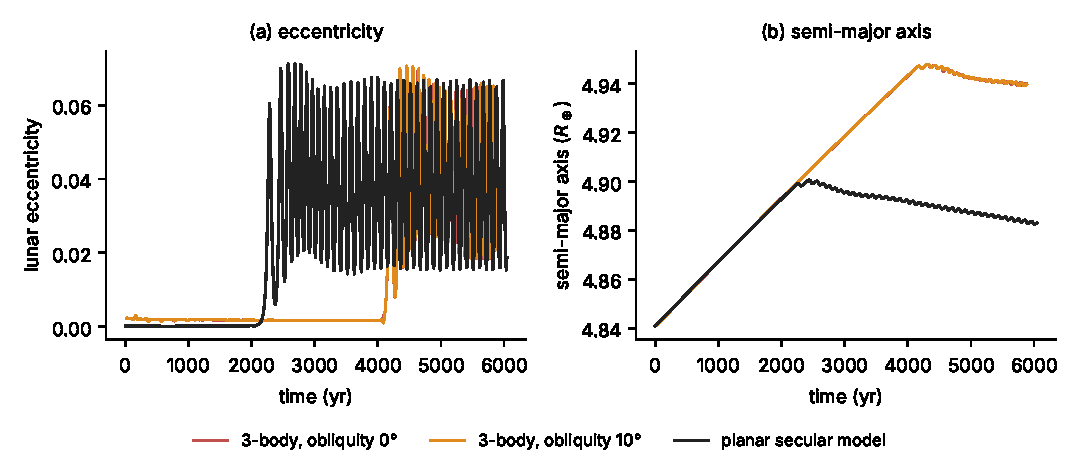
\includegraphics[width=0.95\textwidth]{figures/evection3.pdf}
\caption{Slow case. Eccentricity (a) and semi-major axis (b) of the Moon, three-body calculation (25-year running mean) and planar secular model. The three-body curves are shifted in time, capture taking place at a slightly larger semi-major axis, but their amplitude is the same.\label{fig:evection3}}
\end{figure}

\begin{itemize}
\item \textbf{Slow sweep} (the resonance is crossed over several thousand years). The Moon is captured in the resonance in three bodies as in the secular model, for obliquities of $0^\circ$ and $10^\circ$ and for three lunar tide strengths. The eccentricity oscillates between about $0.015$ and $0.07$ in both models. The removal rate is $6.7\times10^{-4}\,\LEM$ per thousand years in three bodies against $7.2\times10^{-4}$ in the secular model: the three-body calculation gives \textbf{92 to 93\,\%} of the secular rate.
\item The resonance is narrow (about $0.3\,\%$ in semi-major axis). Capture takes place at a slightly larger semi-major axis in three bodies ($4.945\,\Rt$ against $4.90\,\Rt$), hence the shift in figure~\ref{fig:evection3}.
\item \textbf{Fast sweep.} Capture is rare in both models (maximum eccentricity at most $0.04$ in the eight three-body realisations). Capture therefore depends on the sweep speed, and the two models agree on this point.
\end{itemize}

The results of the secular model are thus reproduced in three bodies for the slow sweep, with a removal rate 7 to 8\,\% lower. The effect of this gap on the closure shares is tested in appendix~\ref{app:ferm}. The control covers a limited number of cases; it does not cover the whole grid of table~\ref{tab:couple}.

\subsection{Capture duration}

The total removal is approximately the removal rate multiplied by the time during which the Moon stays captured, so the duration is a quantity one needs to know. It was measured in the secular model for $108$ trajectories: contraction time $\tau_c=2\times10^5$, $5\times10^5$ and $10^6$ years, early terrestrial tide of $0.03$, $0.1$ and $0.3\,\%$ of the reference, lunar dissipation $(k_2/Q)_L=3\times10^{-4}$, $10^{-3}$ and $3\times10^{-3}$, and four arrival phases in the resonance. Capture is counted as long as the eccentricity exceeds $0.02$ (step of $500$ years); $\Sigma$ is the angular momentum removed from the system, in units of $\LEM$.

\begin{table}[htbp]
\centering\footnotesize\setlength{\tabcolsep}{5pt}
\caption{Capture duration (in thousands of years) and cumulated removal $\Sigma$ (in $\LEM$), according to the contraction time $\tau_c$, the early terrestrial tide (in \% of the reference) and the lunar dissipation $(k_2/Q)_L$. Each cell groups four arrival phases; minimum / median / maximum are given.\label{tab:duree}}
\begin{tabular}{ccccc}\toprule
$\tau_c$ (yr) & early tide (\%) & $(k_2/Q)_L$ & duration (kyr) & $\Sigma$ ($\LEM$) \\\midrule
$2\times10^5$ & 0.03 & $3\times10^{-4}$ & 137 / 147 / 152 & 0.12 / 0.13 / 0.13\\
$2\times10^5$ & 0.03 & $10^{-3}$ & 42 / 47 / 50 & 0.07 / 0.07 / 0.07\\
$2\times10^5$ & 0.03 & $3\times10^{-3}$ & 7 / 8 / 10 & 0.03 / 0.03 / 0.03\\
$2\times10^5$ & 0.1 & $3\times10^{-4}$ & 2 / 3 / 4 & 0.00 / 0.00 / 0.00\\
$2\times10^5$ & 0.1 & $10^{-3}$ & 54 / 60 / 76 & 0.07 / 0.08 / 0.12\\
$2\times10^5$ & 0.1 & $3\times10^{-3}$ & 19 / 20 / 22 & 0.05 / 0.05 / 0.06\\
$2\times10^5$ & 0.3 & $3\times10^{-4}$ & 6 / 6 / 6 & 0.01 / 0.01 / 0.01\\
$2\times10^5$ & 0.3 & $10^{-3}$ & 0 / 0 / 0 & 0.00 / 0.00 / 0.00\\
$2\times10^5$ & 0.3 & $3\times10^{-3}$ & 0 / 8 / 20 & 0.00 / 0.03 / 0.06\\
\midrule
$5\times10^5$ & 0.03 & $3\times10^{-4}$ & 266 / 270 / 273 & 0.22 / 0.22 / 0.22\\
$5\times10^5$ & 0.03 & $10^{-3}$ & 98 / 102 / 106 & 0.13 / 0.13 / 0.13\\
$5\times10^5$ & 0.03 & $3\times10^{-3}$ & 14 / 15 / 20 & 0.06 / 0.06 / 0.06\\
$5\times10^5$ & 0.1 & $3\times10^{-4}$ & 4 / 130 / 264 & 0.00 / 0.12 / 0.25\\
$5\times10^5$ & 0.1 & $10^{-3}$ & 96 / 112 / 126 & 0.13 / 0.15 / 0.19\\
$5\times10^5$ & 0.1 & $3\times10^{-3}$ & 33 / 41 / 46 & 0.07 / 0.10 / 0.10\\
$5\times10^5$ & 0.3 & $3\times10^{-4}$ & 6 / 7 / 7 & 0.01 / 0.01 / 0.01\\
$5\times10^5$ & 0.3 & $10^{-3}$ & 0 / 45 / 91 & 0.00 / 0.10 / 0.21\\
$5\times10^5$ & 0.3 & $3\times10^{-3}$ & 0 / 12 / 24 & 0.00 / 0.04 / 0.09\\
\midrule
$10^6$ & 0.03 & $3\times10^{-4}$ & 414 / 420 / 434 & 0.30 / 0.30 / 0.30\\
$10^6$ & 0.03 & $10^{-3}$ & 158 / 164 / 170 & 0.19 / 0.19 / 0.19\\
$10^6$ & 0.03 & $3\times10^{-3}$ & 28 / 29 / 31 & 0.10 / 0.10 / 0.10\\
$10^6$ & 0.1 & $3\times10^{-4}$ & 4 / 4 / 4 & 0.00 / 0.00 / 0.00\\
$10^6$ & 0.1 & $10^{-3}$ & 146 / 162 / 178 & 0.18 / 0.20 / 0.26\\
$10^6$ & 0.1 & $3\times10^{-3}$ & 60 / 70 / 76 & 0.12 / 0.16 / 0.19\\
$10^6$ & 0.3 & $3\times10^{-4}$ & 6 / 7 / 8 & 0.01 / 0.01 / 0.01\\
$10^6$ & 0.3 & $10^{-3}$ & 0 / 56 / 117 & 0.00 / 0.13 / 0.27\\
$10^6$ & 0.3 & $3\times10^{-3}$ & 34 / 36 / 40 & 0.09 / 0.10 / 0.11\\
\bottomrule
\end{tabular}
\end{table}

\begin{figure}[htbp]
\centering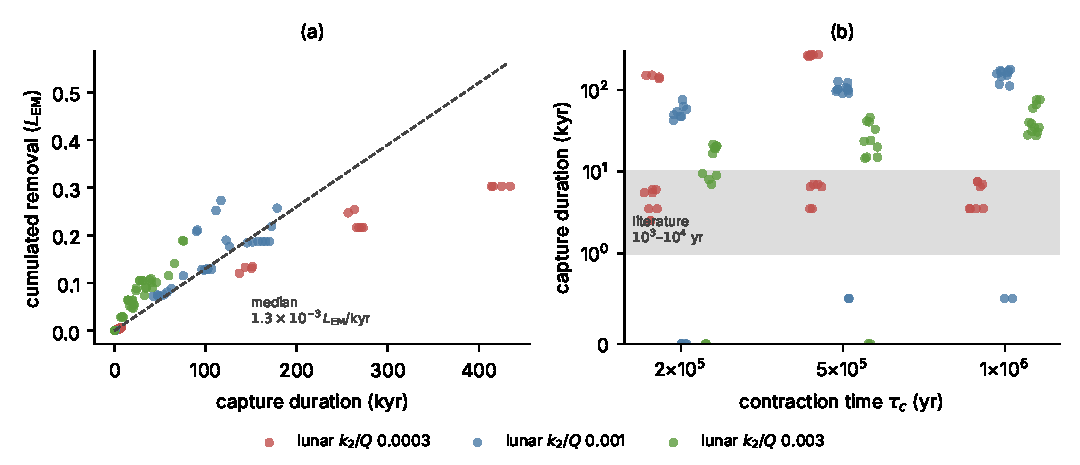
\includegraphics[width=\textwidth]{figures/duree_capture.pdf}
\caption{Capture duration in evection for the $108$ trajectories of table~\ref{tab:duree}. (a)~Cumulated removal against duration; the dashed line is the median rate. (b)~Duration against $\tau_c$; the grey band marks the $10^3$ to $10^4$ year passages reported in the literature.\label{fig:duree}}
\end{figure}

\paragraph{What the grid shows.}
\begin{itemize}
\item Of the $108$ trajectories, $8$ are not captured (maximum eccentricity below $0.02$); all of them have an early tide of $0.3\,\%$. Among the $100$ captured trajectories, the duration ranges from $0.5$ to $435$ thousand years, with a median of $39$ thousand years ($3.5$ at the first decile, $186$ at the last). In all, $38$ trajectories out of $108$ ($35\,\%$) last less than $10^4$ years, non-captures included, and $56$ ($52\,\%$) last $3\times10^4$ years or more.
\item The removal is proportional to the duration: for the captured trajectories its median is $1.3\times10^{-3}\,\LEM$ per thousand years, of the same order as the rate of appendix~\ref{app:evec}. It reaches at most $0.30\,\LEM$, and $0.10\,\LEM$ or more in $44\,\%$ of the trajectories.
\item The duration depends strongly on the early tide. The medians are $102$, $50$ and $6.5$ thousand years for $0.03$, $0.1$ and $0.3\,\%$: the stronger the early tide, the sooner the Moon leaves the resonance. It also grows with $\tau_c$ (medians of $13$, $41$ and $50$ thousand years), but not monotonically with the lunar dissipation: it is the combination of the three parameters that matters, as table~\ref{tab:duree} shows.
\item The maximum eccentricity reached has a median of $0.066$ and a maximum of $0.19$.
\end{itemize}

\paragraph{Comparison with the literature.}
The evection passages reported by \citet{WardCanupRufu2020} and \citet{RufuCanup2020} last of the order of $10^3$ to $10^4$ years and remove a few percent to about ten percent of the angular momentum; \citet{Zahnle2015} find, for slow evolution, near-certain capture but a small eccentricity. In our grid, about half of the captures last $3\times10^4$ years or more, that is at least three times the upper bound of those passages, and they remove more. These durations depend on the early tide and the lunar dissipation, which are posed parameters (section~\ref{sec:couple}), not results: the comparison indicates what these parameters must be for closure to be possible; it does not establish them. The calculation that would fix them is the tide of a soft body, with the viscosity of its material, listed in the programme of table~\ref{tab:programme}.

\section{Budget closure: sensitivity and rebuilt states}
\label{app:ferm}

This appendix extends section~\ref{sec:couple}. Status: \stCalc. Shares of trajectories are grid shares, not probabilities; one trajectory is worth $2.8$ percentage points.

\subsection{Sensitivity to the evection yield}

Appendix~\ref{app:trois} shows that the three-body model gives $92$ to $93\,\%$ of the secular removal rate. To see whether such a gap changes the closure shares, the removal $\Sigma$ of each trajectory of the grid of table~\ref{tab:couple} was rescaled by $f=1$, $0.925$ and $0.85$ (36 trajectories per $\Delta L_B$ and $\tau_c$).

\begin{table}[htbp]
\centering\footnotesize\setlength{\tabcolsep}{4pt}
\caption{Closure shares (\%) for $\varepsilon=0.03;\,0.05;\,0.08;\,0.10\,\LEM$ as a function of the evection yield $f$.\label{tab:sensib}}
\begin{tabular}{ccccc}\toprule
$\tau_c$ (yr) & $\Delta L_B$ & $f=1$ & $f=0.925$ & $f=0.85$ \\\midrule
$3\times10^5$ & 0 & 17 19 33 39 & 6 17 28 33 & 3 14 25 33\\
 & 0.04 & 17 31 47 56 & 22 28 47 56 & 14 22 33 50\\
 & 0.07 & 8 36 44 56 & 11 19 44 56 & 11 17 42 56\\\midrule
$5\times10^5$ & 0 & 11 25 44 50 & 17 31 44 44 & 19 25 31 44\\
 & 0.04 & 6 31 50 75 & 11 39 47 64 & 19 25 44 56\\
 & 0.07 & 22 31 64 69 & 28 39 67 69 & 14 42 56 69\\\midrule
$10^6$ & 0 & 25 25 39 58 & 25 33 39 69 & 8 33 47 50\\
 & 0.04 & 22 25 50 56 & 19 28 47 56 & 22 31 44 64\\
 & 0.07 & 8 33 44 50 & 14 36 50 50 & 14 31 50 61\\\midrule
$2\times10^6$ & 0 & 6 28 50 64 & 8 39 58 67 & 19 33 56 64\\
 & 0.04 & 19 22 33 47 & 22 25 44 50 & 14 25 47 56\\
 & 0.07 & 19 19 31 31 & 19 25 31 42 & 22 25 42 42\\\bottomrule
\end{tabular}
\end{table}

The shares stay in the same range (typically $30$ to $70\,\%$ for $\varepsilon\ge0.08$) and the variations from one column to another, a few trajectories, are of the same order as the grid step; no systematic drift can be read. A removal of $0.04$ to $0.07\,\LEM$ by planet~$B$ gives the highest shares for $\tau_c=5\times10^5$~yr ($64$ to $75\,\%$ at $\varepsilon=0.08$--$0.10$).

\subsection{Rebuilt phase C states}

The coupled budget was redone with four initial states from the phase~C redone with merging on contact (appendix~\ref{app:phaseC}) that retain a Moon: rotation of $6.2$~h (seeds 1 and 2) and $6.4$~h (seeds 0 and 1). Tide and contraction parameters are those of table~\ref{tab:couple}, $\Delta L_B=0$, $288$ trajectories.

\begin{table}[htbp]
\centering\footnotesize\setlength{\tabcolsep}{4pt}
\caption{Budget closure with the rebuilt phase~C states. Shares (\%) for $\varepsilon=0.03;\,0.05;\,0.08;\,0.10\,\LEM$.\label{tab:refondu}}
\begin{tabular}{cccc}\toprule starting state & $\tau_c$ (yr) & share that closes (\%) & Moon lost\\\midrule
6.2 h, seed 1 & $5\times10^5$ & 11 22 28 31 & 0\\ & $10^6$ & 6 22 36 36 & 0\\
6.2 h, seed 2 & $5\times10^5$ & 28 28 36 47 & 0\\ & $10^6$ & 22 36 47 56 & 2\\
6.4 h, seed 0 & $5\times10^5$ & 22 25 47 67 & 0\\ & $10^6$ & 11 36 50 56 & 2\\
6.4 h, seed 1 & $5\times10^5$ & 19 25 44 64 & 0\\ & $10^6$ & 19 31 50 56 & 4\\\bottomrule\end{tabular}
\end{table}

For $\varepsilon=0.08$--$0.10$ the shares range from $28$ to $67\,\%$ depending on the state, within the range obtained with the state of table~\ref{tab:couple} ($39$ to $58\,\%$ at $\Delta L_B=0$). The four rebuilt states therefore close the budget without the starting state having been chosen for that purpose; they do not all do so at the same level, and the spread between states is of the same order as the spread between phase~C seeds.


\section{Phase C: collision speeds, initial rotation and merging thresholds}
\label{app:phaseC}

This appendix extends section~\ref{sec:methode} (paste rule, $H4$). Status: \stCalc, with small samples that the text points out. Phase~C is chaotic: the same seed replayed can give a different result (the mass of the dominant body goes from $0.12$ to $0.41$ lunar mass for $6.0$~h and seed~0), so a single run cannot settle anything.

\subsection{Distribution of collision speeds}

In four runs at $6.0$~h, the relative speed of each of the $768$ collisions was recorded. The median is $2.3$~km\,s$^{-1}$; the quartiles are $1.4$ and $3.5$~km\,s$^{-1}$, $10\,\%$ of the collisions are below $0.9$ and $10\,\%$ above $4.7$~km\,s$^{-1}$. The shares below a threshold are $3\,\%$ ($0.5$), $13\,\%$ ($1$), $43\,\%$ ($2$) and $66\,\%$ ($3$~km\,s$^{-1}$). Only $5.7\,\%$ of the collisions are slower than the escape speed of the colliding pair; they are concentrated in the first thirty days.

\begin{figure}[htbp]
\centering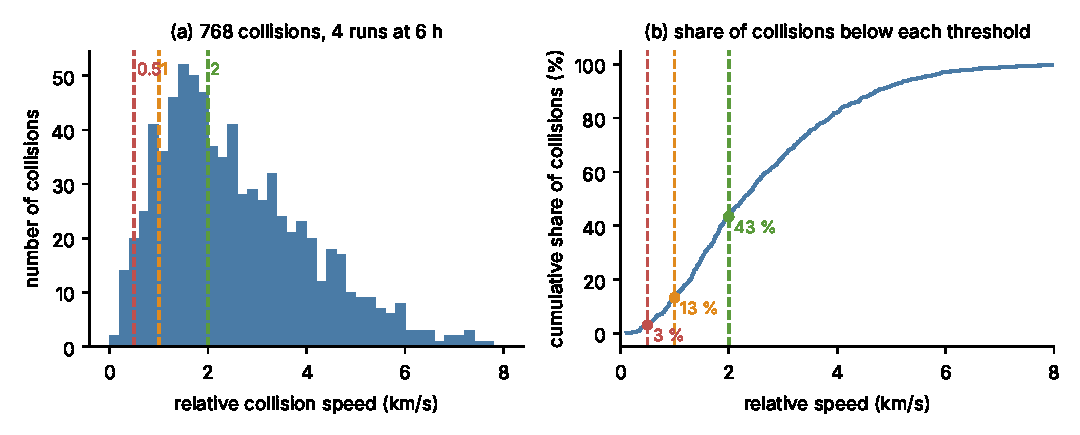
\includegraphics[width=0.95\linewidth]{vrel.pdf}
\caption{Relative speeds of the $768$ collisions (phase~C, $6.0$~h, four runs): histogram (a) and cumulative share below each threshold (b).}
\end{figure}

\subsection{Scan of the initial rotation}

\begin{table}[htbp]
\centering\small
\caption{Phase~C with merging on contact (OMB $=90^\circ$), one to three runs per rotation. The verdict follows the rule of section~\ref{sec:methode}. The ``control'' rows are instrumented replays (collision speeds recorded).\label{tab:rotscan}}
\begin{tabular}{cccccc}\toprule rotation & seed & $M_1$ ($\ML$) & $a_1$ ($\Rt$) & $e_1$ & verdict\\\midrule
6.0 h & 0 & 0.12 & 3.11 & 0.33 & not achieved\\
6.0 h & 0 (control) & 0.41 & 4.55 & 0.15 & not achieved\\
6.0 h & 1 (control) & 0.95 & 3.38 & 0.11 & retained\\
6.2 h & 0 & 0.14 & 2.91 & 0.17 & not achieved\\
6.2 h & 1 & 0.91 & 3.13 & 0.15 & retained\\
6.2 h & 2 & 0.95 & 3.02 & 0.14 & retained\\
6.4 h & 0 & 1.02 & 2.79 & 0.04 & retained\\
6.4 h & 1 & 1.02 & 3.28 & 0.13 & retained\\
6.8 h & 0 & 0.37 & 4.94 & 0.29 & not achieved\\
6.8 h & 1 & 1.09 & 3.09 & 0.10 & retained\\\bottomrule\end{tabular}
\end{table}

Six runs out of ten give a retained Moon, of $0.91$ to $1.09$ lunar mass. For the same rotation, two seeds can give different verdicts; with one to three draws per value, nothing allows us to say that the rotation decides the verdict. Two other $6.0$~h controls, interrupted at $320$ and $85$ days, are not counted.

\subsection{Merging thresholds}

Hypothesis $H4$ (merging on contact) was replaced by a threshold law: two bodies merge if their relative speed is below $v_{\rm crit}$, and bounce otherwise (restitution coefficient $0.3$). The grid compares $v_{\rm crit}=0.5;\,1;\,2$~km\,s$^{-1}$ on four states that retain a Moon with merging on contact (rotations $6.2$~h, seeds 1 and 2, and $6.4$~h, seeds 0 and 1): twelve simulations of $150$ days, compared with merging on contact for the same seeds at the same time.

\begin{table}[htbp]
\centering\small\setlength{\tabcolsep}{4pt}
\caption{Mass $M_1$ of the dominant body (in $\ML$) at $150$ days as a function of the merging threshold; in bold, the cases that meet the retained-Moon criterion ($M_1>0.5$ and $a_1\ge R_{\rm co}$).\label{tab:seuils}}
\begin{tabular}{lccccc}\toprule $v_{\rm crit}$ & 6.2 h s.\,1 & 6.4 h s.\,0 & 6.2 h s.\,2 & 6.4 h s.\,1 & Moons retained\\\midrule
contact & \textbf{0.89} & \textbf{1.00} & \textbf{0.91} & \textbf{1.02} & 4 of 4\\
2 km\,s$^{-1}$ & \textbf{0.73} & 0.17 & \textbf{0.65} & \textbf{0.68} & 3 of 4\\
1 km\,s$^{-1}$ & 0.46 & \textbf{0.52} & 0.39 & 0.37 & 1 of 4\\
0.5 km\,s$^{-1}$ & 0.12 & 0.20 & 0.13 & 0.21 & 0 of 4\\\bottomrule\end{tabular}
\end{table}

\begin{figure}[htbp]
\centering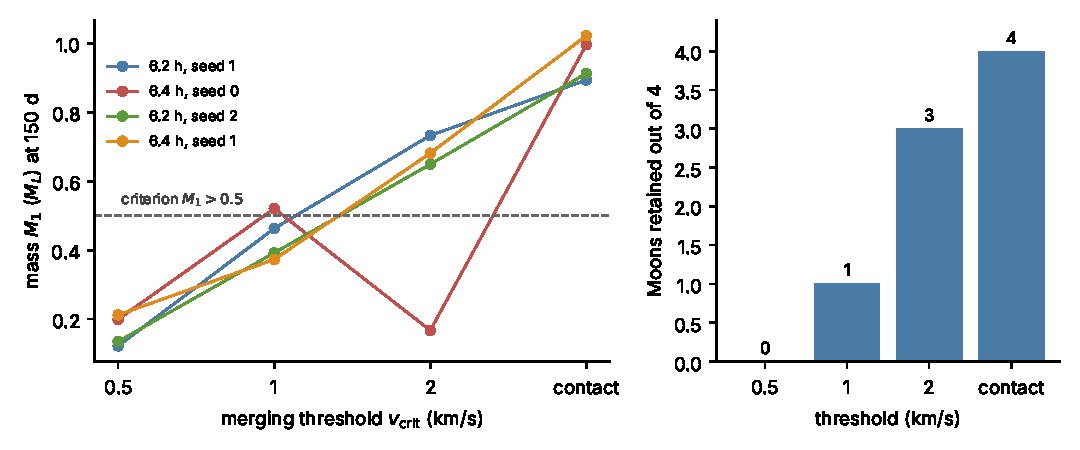
\includegraphics[width=0.95\linewidth]{seuils.pdf}
\caption{Mass of the dominant body (a) and number of retained Moons (b) as a function of the merging threshold, for the four states.}
\end{figure}

In this sample the retained mass increases markedly when the threshold goes from $0.5$ to $2$~km\,s$^{-1}$, with one exception (rotation $6.4$~h, seed~0, where the $2$~km\,s$^{-1}$ threshold scatters the Moon to $a_1=7.9\,\Rt$). A Moon is retained in three states out of four with a threshold of $2$~km\,s$^{-1}$, in one out of four at $1$ and in none at $0.5$. Forming a Moon therefore requires efficient accretion up to about $2$~km\,s$^{-1}$ here; it does not require merging at every speed: with a threshold of $2$~km\,s$^{-1}$, more than half of the collisions ($57\,\%$) bounce, and the Moon is still retained in three cases out of four.

\subsection{Limits}

One simulation per cell; only $150$ days (the structure is set in the first months, which we did not check at $365$ days for each state); restitution coefficient fixed at $0.3$ and not tested; threshold carried by relative speed alone, with no temperature dependence. The preliminary $6.0$~h tests, one draw per threshold, did not succeed; $6.0$~h is also the most uncertain rotation with merging on contact (table~\ref{tab:rotscan}). The speed--temperature map of accretion remains to be drawn: it requires a collision law that depends on temperature, which the code does not contain. The complete outputs are in the package described in appendix~\ref{app:repro}.



\section{Glossary}

\begin{description}[leftmargin=3.2cm,style=nextline,itemsep=2pt]
\item[Obliquity] angle between the rotation axis of a planet and the normal to its orbit.
\item[Planet~$B$] the second rocky planet ($0.95$ Earth mass) whose flyby, by gravity alone, redistributes the disk.
\item[Proto-Earth] the Earth before the formation of the Moon: hot, soft, swollen.
\item[Soft body] pasty material, neither liquid nor cold solid, whose deformation under the tide dissipates energy.
\item[Roche limit] distance inside which the tide of the planet tears apart a fluid body.
\item[Corotation radius] distance at which a body orbits as fast as the Earth rotates; beyond it, the tide pushes the body away, inside it pulls it in.
\item[Retrograde] against the rotation of the Earth.
\item[Phases A, B, C] existence of the disk (A), flyby (B), assembly and evolution (C).
\item[$\LEM$] angular momentum of the present Earth--Moon system, $3.5\times10^{34}$~kg\,m$^2$\,s$^{-1}$.
\item[$k_2/Q$] measure of the tidal dissipation of a body: the larger it is, the more the body turns the tide into heat.
\item[Evection] resonance between the precession of the perigee of the satellite and the apparent motion of the Sun, which removes angular momentum from the system.
\item[Secular] qualifies a calculation that averages over the fast motions to follow the slow evolution.
\end{description}

\bibliographystyle{unsrtnat}
\bibliography{refs}


\end{document}
